%% Преамбула TeX-файла

% 1. Стиль и язык
\documentclass[utf8x, 14pt]{G7-32} % Стиль (по умолчанию будет 14pt)

% Остальные стандартные настройки убраны в preamble.inc.tex.
\sloppy

% Настройки стиля ГОСТ 7-32
% Для начала определяем, хотим мы или нет, чтобы рисунки и таблицы нумеровались в пределах раздела, или нам нужна сквозная нумерация.
\EqInChapter % формулы будут нумероваться в пределах раздела
\TableInChapter % таблицы будут нумероваться в пределах раздела
\PicInChapter % рисунки будут нумероваться в пределах раздела

% Добавляем гипертекстовое оглавление в PDF
\usepackage[
bookmarks=true, colorlinks=true, unicode=true,
urlcolor=black,linkcolor=black, anchorcolor=black,
citecolor=black, menucolor=black, filecolor=black,
]{hyperref}

% Изменение начертания шрифта --- после чего выглядит таймсоподобно.
% apt-get install scalable-cyrfonts-tex

\IfFileExists{cyrtimes.sty}
    {
        \usepackage{cyrtimespatched}
    }
    {
        % А если Times нету, то будет CM...
    }

\usepackage{graphicx}   % Пакет для включения рисунков

% С такими оно полями оно работает по-умолчанию:
%\RequirePackage[left=30mm,right=10mm,top=20mm,bottom=20mm,headsep=0pt]{geometry}
% Если вас тошнит от поля в 10мм --- увеличивайте до 20-ти, ну и про переплёт не забывайте:
%\geometry{right=10mm}
%\geometry{left=30mm}


% Пакет Tikz
\usepackage{tikz}
\usetikzlibrary{arrows,positioning,shadows}

% Произвольная нумерация списков.
\usepackage{enumerate}

% ячейки в несколько строчек
\usepackage{multirow}

% itemize внутри tabular
\usepackage{paralist,array}

% псевдокод
\usepackage{algorithm2e}

\SetKwInput{KwData}{Исходные параметры}
\SetKwInput{KwResult}{Результат}
\SetKwInput{KwIn}{Входные данные}
\SetKwInput{KwOut}{Выходные данные}
\SetKwIF{If}{ElseIf}{Else}{если}{тогда}{иначе если}{иначе}{конец условия}
\SetKwFor{While}{пока}{выполнять}{конец цикла}
\SetKw{KwTo}{от}
\SetKw{KwRet}{возвратить}
\SetKw{Return}{возвратить}
\SetKwBlock{Begin}{начало блока}{конец блока}
\SetKwSwitch{Switch}{Case}{Other}{Проверить значение}{и выполнить}{вариант}{в противном случае}{конец варианта}{конец проверки значений}
\SetKwFor{For}{цикл}{выполнять}{конец цикла}
\SetKwFor{ForEach}{для каждого}{выполнять}{конец цикла}
\SetKwRepeat{Repeat}{повторять}{до тех пор, пока}
\SetAlgorithmName{Алгоритм}{алгоритм}{Список алгоритмов}


% Настройки листингов.
\ifPDFTeX
% 8 Листинги

\usepackage{listings}
% Значения по умолчанию
\lstset{
  basicstyle= \footnotesize,
  breakatwhitespace=true,% разрыв строк только на whitespacce
  breaklines=true,       % переносить длинные строки
%   captionpos=b,          % подписи снизу -- вроде не надо
  inputencoding=koi8-r,
  numbers=left,          % нумерация слева
  numberstyle=\footnotesize,
  showspaces=false,      % показывать пробелы подчеркиваниями -- идиотизм 70-х годов
  showstringspaces=false,
  showtabs=false,        % и табы тоже
  stepnumber=1,
  tabsize=4,              % кому нужны табы по 8 символов?
  frame=single
}

% Стиль для псевдокода: строчки обычно короткие, поэтому размер шрифта побольше
\lstdefinestyle{pseudocode}{
  basicstyle=\small,
  keywordstyle=\color{black}\bfseries\underbar,
  language=Pseudocode,
  numberstyle=\footnotesize,
  commentstyle=\footnotesize\it
}

% Стиль для обычного кода: маленький шрифт
\lstdefinestyle{realcode}{
  basicstyle=\scriptsize,
  numberstyle=\footnotesize
}

% Стиль для коротких кусков обычного кода: средний шрифт
\lstdefinestyle{simplecode}{
  basicstyle=\footnotesize,
  numberstyle=\footnotesize
}

% Стиль для BNF
\lstdefinestyle{grammar}{
  basicstyle=\footnotesize,
  numberstyle=\footnotesize,
  stringstyle=\bfseries\ttfamily,
  language=BNF
}

% Определим свой язык для написания псевдокодов на основе Python
\lstdefinelanguage[]{Pseudocode}[]{Python}{
  morekeywords={each,empty,wait,do},% ключевые слова добавлять сюда
  morecomment=[s]{\{}{\}},% комменты {а-ля Pascal} смотрятся нагляднее
  literate=% а сюда добавлять операторы, которые хотите отображать как мат. символы
    {->}{\ensuremath{$\rightarrow$}~}2%
    {<-}{\ensuremath{$\leftarrow$}~}2%
    {:=}{\ensuremath{$\leftarrow$}~}2%
    {<--}{\ensuremath{$\Longleftarrow$}~}2%
}[keywords,comments]

% Свой язык для задания грамматик в BNF
\lstdefinelanguage[]{BNF}[]{}{
  morekeywords={},
  morecomment=[s]{@}{@},
  morestring=[b]",%
  literate=%
    {->}{\ensuremath{$\rightarrow$}~}2%
    {*}{\ensuremath{$^*$}~}2%
    {+}{\ensuremath{$^+$}~}2%
    {|}{\ensuremath{$|$}~}2%
}[keywords,comments,strings]

% Подписи к листингам на русском языке.
\renewcommand\lstlistingname{\cyr\CYRL\cyri\cyrs\cyrt\cyri\cyrn\cyrg}
\renewcommand\lstlistlistingname{\cyr\CYRL\cyri\cyrs\cyrt\cyri\cyrn\cyrg\cyri}

\else
\usepackage{local-minted}
\fi

% Полезные макросы листингов.
% Любимые команды
\newcommand{\Code}[1]{\textbf{#1}}


\begin{document}

\frontmatter % выключает нумерацию ВСЕГО; здесь начинаются ненумерованные главы: реферат, введение, глоссарий, сокращения и прочее.

% Команды \breakingbeforechapters и \nonbreakingbeforechapters
% управляют разрывом страницы перед главами.
% По-умолчанию страница разрывается.

% \nobreakingbeforechapters
% \breakingbeforechapters
титульник
\newpage
тз
\newpage
тз
\newpage
план
\newpage
% Также можно использовать \Referat, как в оригинале
\begin{abstract}
РПЗ n страниц, p рисунка, q таблиц, t источников.

Объектом исследования данной работы являются музыкальные произведения.
Целью рабоы является разработка метода автоматизированного выделения голосовой составляющей из музыкальной композиции.

Задачи:

\begin{itemize}
	\item анализ предметной области;
	\item анализ методов выделения вокальной партии из музыкальных композиций;
	\item разработка собственного метода на основании проанализированных;
	\item разработка программного комплекса, реализующего выбранный метод;
	\item анализ эффективности работы программного продукта.
\end{itemize}

Способы применения программного продукта: программный продукт может применяться для дальнейшей разработки выделения компонентов сведенного аудио сигнала, выделения голосовой составляющей из песен для автоматизированного создания текста, выделения голосовой составляющей из аудио дорожки видеофайла для улучшения автоматизированной генерации субтитров. 
\end{abstract}

%%% Local Variables: 
%%% mode: latex
%%% TeX-master: "rpz"
%%% End: 


\tableofcontents

\Defines % Необходимые определения. Вряд ли понадобться
В настоящей работе используются следующие термины с соответствующими
определениями.
\begin{description}
\item[Дискретизация] преобразование непрерывного информационного множества аналоговых сигналов в дискретное множество.
\item[Музыкальное произведение] последовательность сочетаний звуков.
\item[Звук] физическое явление, представляющее собой распространение в виде упругих волн механических колебаний в твёрдой, жидкой или газообразной среде.
\item[Колебания] повторяющийся в той или иной степени во времени процесс изменения состояний системы около точки равновесия. Колебания характеризуются частотой, фазой и амплитудой.
\item[Частота] физическая величина, характеристика периодического процесса, равна количеству повторений или возникновения событий в единицу времени. Единица измерения -- герцы (Гц).
\item[Фаза] аргумент периодической функции, описывающей колебательный
или волновой процесс.
\item[Амплитуда] максимальное значение смещения или изменения перемен­
ной величины от среднего значения при колебательном или волновом движении.

Применительно к музыке вместо общего термина <<звук>> используют более конкретный термин <<музыкальный звук>>.
\item[Музыкальный звук] это звук определённой высоты, использующийся
как материал для создания музыкальных сочинений. Для письменной фиксации му­зыкальных звуков используется нотация. Наиболее распространённые формы записи высотных значений музыкальных звуков – латинская буквенная (C, D, E, F, G, A, B/H) или слоговая (до, ре, ми, фа, соль, ля, си) нотация. В данной работе для обозначения музыкальных звуков используется латинская буквенная нотация с указанием номера октавы.
\item[Нота] музыкальный звук или его письменная запись.

Далее понятие <<звук>> используется в смысле музыкального звука.

\item[Аккомпанемент] сопровождение одним или несколькими инструментами, а также оркестром сольной партии (певца, инструменталиста, хора и других). Сопроводителя называют аккомпаниатором. Аккомпанементом также называют гармоническое и ритмическое сопровождение основной мелодии, голоса.
\item[Вокал (или пение)] исполнение мелодии с помощью голоса человека.
\item[Тембр] (обертоновая) окраска звука, <<качество тона>>.
\item[Рефакторинг] процесс изменения внутренней структуры программы, не затрагивающий её внешнего поведения и имеющий целью облегчить понимание её работы.
\item[Цифровая звуковая рабочая станция] электронная или компьютерная система, предназначенная для записи, хранения, редактирования и воспроизведения цифрового звука. Предусматривает возможность выполнения на ней законченного цикла работ, от первичной записи до получения готового результата.
\end{description}

%%% Local Variables:
%%% mode: latex
%%% TeX-master: "rpz"
%%% End:

\Abbreviations %% Список обозначений и сокращений в тексте
\begin{description}
\item[АИС] Автоматизированная информационная система. Но надо протестировать длинные строки в определениях.
\end{description}

%%% Local Variables:
%%% mode: latex
%%% TeX-master: "rpz"
%%% End:


\Introduction

Тут будет крассиво введение.

\mainmatter % это включает нумерацию глав и секций в документе ниже

\chapter{Аналитический раздел}
\label{cha:analysis}

Выделение голосовой составляющей из аудио сигнала является частным случаем задачи разделения комбинации аудио сигналов на составляющие. Музыкальное произведение может быть записано как с использованием нескольких микрофонов, захватывающих разные источники, при этом изоляция источников будет ограничена, либо с использованием выделенной на каждый источник. Все записанные сигналы в последствии проходят процесс сведения для получения итоговой аудио записи. Тем самым конечный аудио сигнал можно представить в виде суммы отдельных источников с приминением фильтров к каждому источнику.

Математически это можно записать как:

\begin{equation}
 x(t) = \sum_{j=1}^{J} \sum_{\tau=-\infty}^{\infty} a_{j}(t-\tau, \tau)s_j(t-\tau)
 \label{anal:result-signal}
\end{equation}

где 

\begin{itemize}
	\item $x$ -- итоговый аудио сигнал;
	\item $s_j$ -- сигнал источника;
	\item $J$ -- количество источников;
	\item $a_j$ -- фильтр, примененный к источнику в процессе сведения.
\end{itemize}

Если приминяемые фильтры являются линейными, то итоговый сигнал представляет собой линейную комбинацию. С другой стороны, к итоговому сигналу так же могут быть применены фильтры. С этой точки зрения сведенный сигнал перестает быть линейной суммой отдельных источников. 

Тем самым, итоговая запись, в контексте задачи выделения аудио источников, может быть определена по следующим признакам\cite{[Chandna}:

\begin{enumerate}
	\item Количество используемых во время записи источников аудио сигнала. Источники могут быть записаны как отдельно, с помощью выделенных линий звукозаписи либо нескольких микровонов, так и при помощи одного микрофона, захватывающего все звуки одновременно. С понижением количества звукозаписывающих устройств повышается смешанность отдельных аудио сигналов и влияние на них шумов.
	\item Количество примененных к итоговому аудио сигналу эффектов. С учетом итоговых фильтров формула \ref{anal:result-signal} принимает вид:
	\begin{equation}
	x(t) =\prod_{k=1}^K \psi_{k}(t) \sum_{j=1}^{J} \sum_{\tau=-\infty}^{\infty} a_{j}(t-\tau, \tau)s_j(t-\tau)
	\label{anal:filtered-signal}
	\end{equation}
	где $\psi_{k}(t), k=1б ..., K$ -- применяемые к итоговому сигналу фильтры.
	Исходя из формулы, применение фильтров к итоговому сигналу усложняет задачу выделения аудио источников.
	\item Изменение положения звукозаписывающих устройств во время записи. Микрофоны, ведущие запись, могут быть статичными, находясь в закрепленном состоянии, либо перемещаться, например от одного источника к другому. Второй случай оказывает непосредственное влияние на сигналы аудио источников, добавляя шумы и изменяя уровень сигнала.
\end{enumerate}

Эта работа будет сфокусирована на обработке записей без итоговых фильтров, источники которых были записаны независимо друг от друга без изменений положения звукозаписывающих устройств.

\section{Цифровое представление аудио сигналов}

Звук имеет три основных характеритичесих параметров: амплитуда, частота и фаза. Две последнии характеристики являются функциями времени, в то время как амплитуда определяет динамический диапозон. По этому в цифровом представлении аудио сигнала записываются изменения аплитуды как функция времени. Тем самым процесс отцифровки аналогового аудио сигнала является записью мгновенных амплитудных значений (дискретизация по амплитуда) в постоянные моменты времени (дискретизация по времени). Графическое представление дискретизации аналогового сигнала представлено на рисунке \ref{anal:atob}.

\begin{figure}
	\centering
	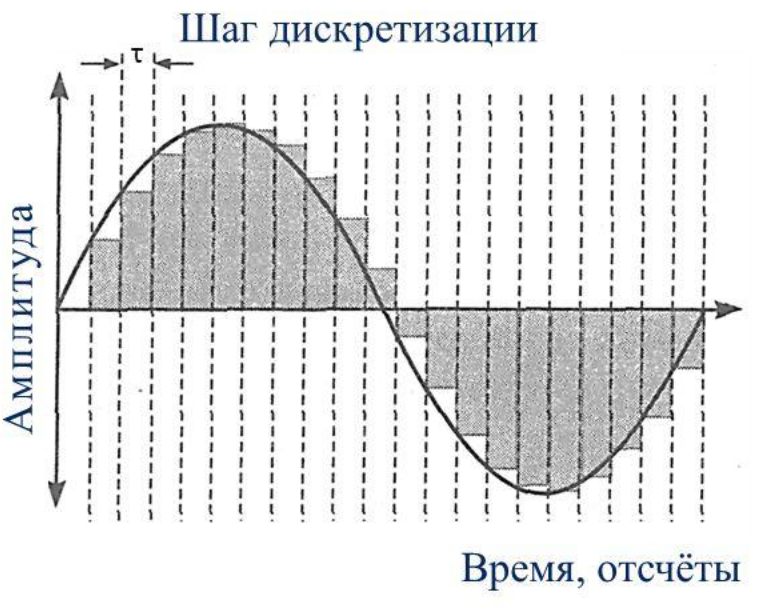
\includegraphics[width=0.5\textwidth]{inc/img/analog-to-bin.png}
	\caption{Дискретизация аналогового сигнала}
	\label{anal:atob}
\end{figure}

Для определения периода записи амплитудных значений задается частота дискретизации. 

Существует теорема Котельникова\cite{Bikkenin}, утверждающая, что <<любую функцию $F(t)$, состоящую из частот от 0 до $f_1$, можно непрерывно передавать с любой точностью при помощи чисел, следующих друг за другом через $1/(2f_1)$ секунд>>.

При максимальной воспринимаемой человеческим ухом частоте в 20 кГц, по теореме Котельникова минимальная необходимая частота дискретизации должна быть 40 кГц.

Стандартная частота дискретизации аудио сигнала составляет 44,1 кГц, максимальная -- 192 кГц.

Для определения максимального значения амплитуды используется значение квантования (или разрядность), задающаяся в битах. В зависимости от используемого формата разрядность может быть 1, 8, 16, 24 и 32 бит.

В данной работе будут использоваться wav-файлы (сокращение Waveform Audio File Format). Формат WAVE был разработан корпорацией Майкрософт, является контейнером для хранения и записи оцифрованных аудиопотоков. Представляет из себя сжатый формат, отличается отсутствием потери качества и основан на расширении RIFF. Структура wav-файлов имеет чёткую форму, описанную в стандарте \cite{wav}.

\section{Существующие методы выделения источников}

Методы выделения источников делятся на две основные категории\cite{mansour:hal-00802445}.

\begin{itemize}
	\item Слепое выделение. Методы, относяющиеся к данной категории, обрабатывают смесь аудио сигналов без помощи, или с минимальным количеством, информации об источниках и методах их сведения. Наиболее популярные из этих алгоритмов используют (предполагаемую) статистическую независимость исходных сигналов. Примером являются Метод главных компонент \cite{Lopez} \cite{Dadula}, Факторизация неотрицательных матриц. С ростом количества исследований в области нейронных сетей возникла идея применения методов глубинного обучения в задачах выделения источников. Работы по данной теме были сфокусированы на таких сетях как Глубинные и Сверточные нейронные сети.
	\item Информированное выделение. Для данной категории методов предполагается наличие предварительной информации об исходных сигналах, в форме MIDI, партитуры или другом виде представления музыки\cite{Miron}. Целью данной работы не является изучение информированного выделения, потому детального описания представлено не будет.
\end{itemize}

Данная работа будет сфокусирована на методах слепого выделения.

\subsection{Метод главных компонент}
Метод главных компонент (англ. Principal Component Analysis) и анализ независимых компонент (англ. Independent Component Analysis) -- это статистические способы уменьшения размерности данных, который являлся объектом для исследований в области выделения аудио источников \cite{Lopez} \cite{Dadula}.

Основная идея этоих метода заключается в том, чтобы проецировать данные из временных рядов, таких как аудиозапись, в новые системы отсчета, которые основаны на некотором статистическом критерии. Эти оси являются статистически независимые в отличие от преобразования Фурье, где данные временной области проецируются на оси частот, которые могут перекрываться. Частотные оси в преобразовании Фурье остаются неизменными независимо от анализируемой части, тогда как в методе главных компонент и анализе независимых компонент оси являются динамическими и различны для каждой анализируемой части. После нахождения, оси, на которые происходит проецирование, могут быть разделены и инвертированы для нахождения источников, представленных в исходном сигнале.

Формулу \ref{anal:result-signal} можно представить в виде:

\begin{equation}
x(t) = As(t)
\end{equation}

где

\begin{itemize}
	\item $A$ -- квадратная матрица, состоящая из коэффициентов исходного сигнала.
	\item $s(t)$ -- множество сигналов выделяемых источников.
\end{itemize}

Имея оценку матрицы $A$ можно получить искомые источники с помощью обратной ей матрицы $W$:

\begin{equation}
y(t) = Wx(t)
\end{equation}

В рамках задачи слепого выделения источников данный метод сводится к серии матричных произведений, представляющих свобой фильтры. В общем случае входной сигнал $X$ размерности $N$ из $M$ образцов (представляется матрицей размерности $NxM$) может быть приведен к сигналу $Y$ с использованием матрицы преобразования $W$ размерности $NxN$ как $Y^T = WX^T$. Такое преобразование проецирует сигнал на разные оси основываясь на матрице преобразования. Если размер полученного сигнала равен размер исходного сигнала, то преобразование называется ортогональным и оси перпендикулярны.

Данный метод является иттеративным с фиксированной точкой. В нем применяется нелиейная функция $g(y) = th(a * y)$, которая применяется к матрице разделения $W$, которая пересчитывается на каждом шаге.

Входные данные для данного метода должны быть обработаны следующей последовательностью действий:

\begin{enumerate}
	\item центрирование по среднему значению;
	\item нормализация по дисперсии;
	\item ортоганализация.
\end{enumerate}

После этого случайным образом выбирается начальное значение вектора $W$, которое уточняется с помощью следующих иттеративных шагов:

\begin{enumerate}
	\item Обновление $W$ по формуле:
	
	\begin{equation}
		w = E\{zg(w^Tz)\} - E\{g'(w^Tz)\}w
	\end{equation}
	
	где $z$ -- обработанные входные данные.
	\item $w = \frac{w}{|| w ||}$
\end{enumerate}

Выполняются до достижения сходимости.

\subsection{Факторизация неотрицательных матриц}

Факторизация неотризательных матриц (англ. Non-Negative Matrix Factorization) широко использовалась в области выделения источников в прошлом. Основная идея данного метода заключается в представлении матрицы $Y$ в виде комбинации базиса $B$ и активационного усиления $G$ как $Y=BG$. Базовый вектор предстовляет частотную характеристику источника в заданный момент времени, а вектор $G$ представляет усиление частот в любой момент времени. Таким временем $G$ является горизонтальным вектором вдоль времени.

В контексте задачи выделения аудио источников, если исходный сигнал является объединением двух источников, $S_1$ и $S_2$, так, что $Y = S_1 + S_2$, и базисные вектора двух источников вычисляются как $B_1$ и $B_2$, то исходный сигнал можно представить как $Y = B_1 G_1 + B_2 G_2$, где $G_1$ и $G_2$ -- соответсвующие активанционные усиления для двух источников, представленные в разные моменты времени. 

Для применения факторизации неотрицательных матриц необходимо, чтобы сигнал представлял из себя линейную комбинацию базисных векторов. Для $K$ источников:

\begin{equation}
X_{i,j} = \sum_{k=1}^{K} B_{i,k} G_{k, j}
\end{equation}

Расхождение между $X$ и $BG$ должно быть минимизировано, чтобы гарантировать, что найденные аудио источники представляют в комбинации исходный сигнал:

\begin{equation}
{B, G} = argmin_{B, G >= 0} D (X, BG)
\end{equation}

где $D$ является функцией расхождения, которая может быть:

\begin{enumerate}
	\item среднеквадротичным отклонением:
	\begin{equation}
	D (A, B) = ||A-B||^2 = \sum_{ij}(A_{ij} - B_{ij})^2
	\label{anal:mse}
	\end{equation}
	\item дивергенцией Кулбека-Лейблера:
	\begin{equation}
		D (A, B) = \sum_{ij} (A_{ij} \log\frac{A_{ij}}{B_{ij}} - A_{ij} + B_{ij})
		\label{anal:kl}
	\end{equation}
\end{enumerate}

Для этой дивергенции применяется алгоритм мультипликативного обновления \cite{DLee}:

\begin{enumerate}
	\item Вектора $B$ и $G$ заполняются случайными значниями.
	\item Вычисление нового значение $B$: 
	
	Для евклидова расстояния:
	\begin{equation}
	B \leftarrow B \frac{XG^T}{(BG)G^T}
	\end{equation}
	
	Для дивергенции Кулбека-Лейблера:
	\begin{equation}
	B \leftarrow B \frac{ (\frac{X}{BG}) G^T}{1G^T}
	\end{equation}
	\item Вычисление нового значения $G$:
	
	Для евклидова расстояния:
	\begin{equation}
	G \leftarrow G \frac{B^T X}{B^T (BG)}
	\end{equation}
	
	Для дивергенции Кулбека-Лейблера:
	\begin{equation}
	G \leftarrow G \frac{B^T \frac{X}{BG}}{B^T1}
	\end{equation}
\end{enumerate}

Эти действия посторяются предопределенное количество раз, либо до момента достижения дивергенции определенного минимума.

После нахождения магнитуды источника, сигнал можно получить при помощи фазовой характеристики исходного сигнала. 

Работа данного метода зависит от задаваемых начальных условий, зависимых от числа источников и фильтров, примененных к итоговому сигналу.

\subsection{Адаптивный метод FASST}

Адаптивный метод FASST (англ. Flexible Audio Source Separation Toolbox) являются модификацией метода факторизации неотрицательных матриц, основанный на обобщенном EM-алгоритме (англ. Generalized expectation-maximization (GEM) algorithm) \cite{ozerov}. 

Суть данного метода заключается в обобщении реализации, гибкой для разных случаев начальных условий. Каждый выделяемый источник представляется в виде модели возбуждающего фильтра:

\begin{equation}
V_j = V_j^{ex} \bigodot V_j^{ft}
\end{equation}

где $V_j^{ex}$ представляет спектральный возбудитель мощности и $V_j^{ft}$ представляет спектральный фильтр мощности, $\bigodot$ означает поэлементное умножение матриц.

В дальнейшем $V_j^{ex}$ определяется в качестве суммы спектральных шаблонов $E_j^{ex}$, модулированных 	временными коэффициентами $P_j^{ex}$. Эти параметрами являются аналогами базисного вектора и активационного усиления в методе факторизации неотрицательных матриц. Тем самым $V_j^{ex}$ можно переписать как:
\begin{equation}
V_j^{ex} = E_j^{ex}P_j^{ex}
\end{equation}

Спектральные шаблоны представляются в виде линейной комбинации произведения узкополосных спектральных шаблонов $W_j^{ex}$ и неотрицательных весов $U_j^{ex}$.

Временные коэффициенты представляются в виде линейной комбинации произведения кратковременных шаблонов $H_j^{ex}$ и $G_j^{ex}$.

В итоге можно записать:

\begin{equation}
V_j = (W_j^{ex}U_j^{ex}G_j^{ex}H_j^{ex}) \bigodot (W_j^{ft}U_j^{ft}G_j^{ft}H_j^{ft})
\end{equation}

Эти шаблоны оцениваются для каждого источника с помощью GEM алгоритма, с использованием алгоритма мультипликативного обновления \cite{DLee}.

\subsection{Методы, использующие нейронные сети}

Идея применения методов машинного обучения в задачах разделения аудио источников возникла после успешных использований нейронных сетей в других областях, в частности обработки изображений \cite{[Krizhevsky}. Для решения данной задачи наиболее широко рассматривались глубокие\cite{[Grais} и сверточные\cite{[Chandna} нейронные сети.

\subsubsection{Общий принцип работы нейронный сетей}

Нейронная сеть -- система обработки информации, вдохновленная нервной системой человека\cite{Grossberg}. Подобно нервной системе, искусственные нейронные сети состоят из соединения узлов, называемых нейронами. Каждый нейрон получает входной сигнал, обрабатывает информацию во входном сигнале и дает выход. Эти нейроны содержат параметры, которые должны быть оптимизированы с помощью тренировочного набора, который имеет истинные результирующие значения. После обучения сеть может использоваться для ввода данных с целью получения результатов для тестирования и будущего использования. Схема простой нейронной сети представлена на рисунке \ref{anal:simple-nn} и состоит из трех вертикальных слоев:

\begin{figure}
	\centering
	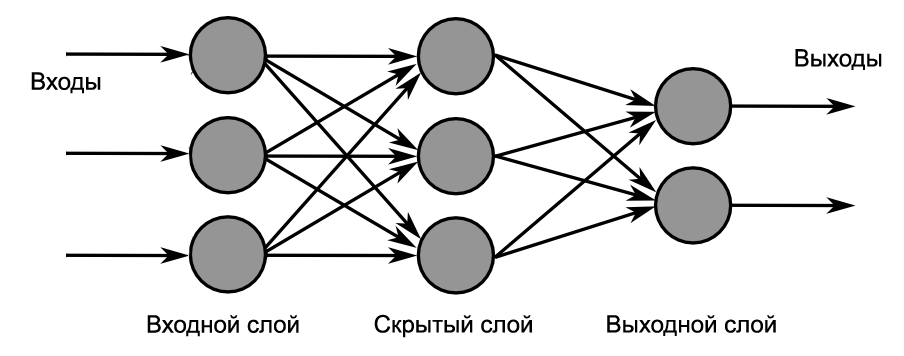
\includegraphics[width=0.8\textwidth]{inc/img/simple-nn.png}
	\caption{Схема простой нейронной сети}
	\label{anal:simple-nn}
\end{figure}

\begin{itemize}
	\item Входной слой -- распределение входных сигналов остальным нейронам. Нейроны этого слоя не производят никаких вычислений.
	\item Скрытый слой -- принимает сигналы с предыдущего слоя, обрабатывает поулченую информацию и передает результат следующему слою.
	\item Выходной слой -- выопляет схожие со скрытым слоем функции за исключением того, что результатом работы выходного слоя является результат работы всей нейронной сети.
\end{itemize}

Каждый слой состоит из нейронов, каждый из которых можно описать математически с помощью его параметров:

\begin{itemize}
	\item Вектор входных данных $X$, состоящий из значений $x_1, ..., x_n$.
	\item Порогове число $b$, является константой, добавляющееся к входному вектору.
	\item Вектор входных весов $W$, состоящий из значений $w_1, ..., w_n$.
	\item Нелинейная активационная функция $\sigma$, которая может быть:
	\begin{itemize}
		\item Гиперболический танцгенс (рис. \ref{anal:th}):
		
		\begin{equation}
			\sigma(x) = \frac{e^x - e^{-x}}{e^x + e^{-x}}
		\end{equation}
		
		\begin{figure}
			\centering
			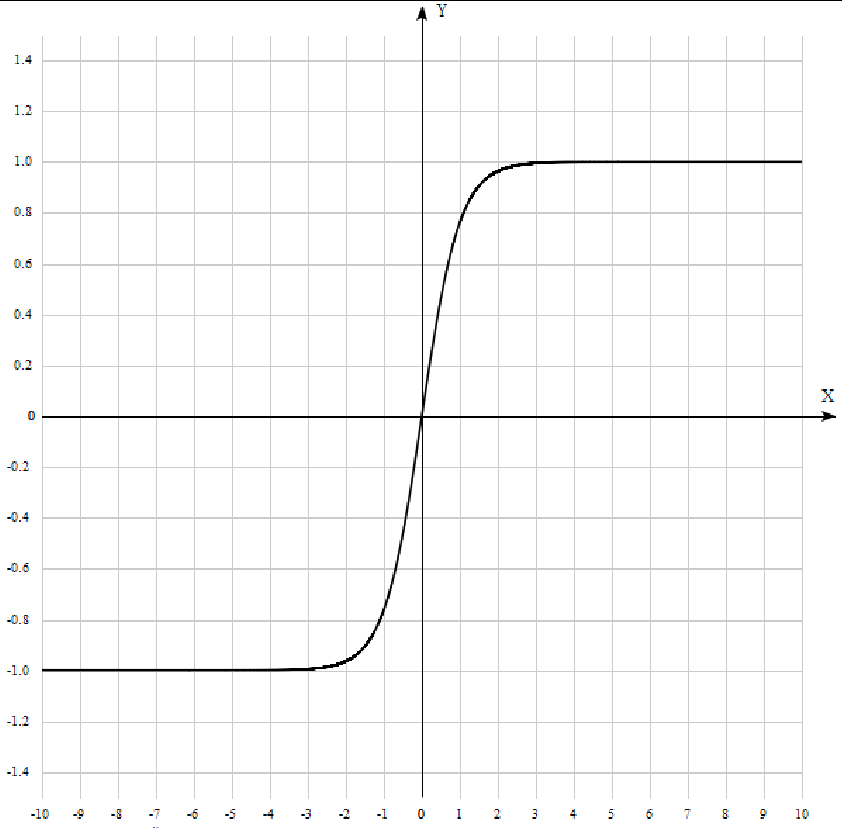
\includegraphics[width=0.5\textwidth]{inc/img/th.png}
			\caption{График гиперболического тангенса}
			\label{anal:th}
		\end{figure}
		
		\item Сигмоида (рис. \ref{anal:sigm}):
		
		\begin{equation}
		\sigma(x)=\frac{1}{1+e^{-x}}
		\end{equation}
		
		\begin{figure}
			\centering
			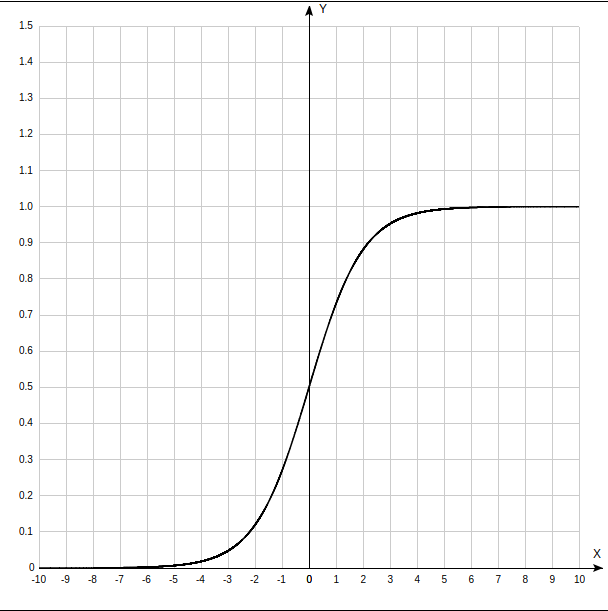
\includegraphics[width=0.5\textwidth]{inc/img/sigmoid.png}
			\caption{График сигмоиды}
			\label{anal:sigm}
		\end{figure}
		
		\item Линейная функция активации ReLU (рис. \ref{anal:relu}):
		
		\begin{equation}
		\sigma(x) = max(0, x)
		\end{equation}
		
%		\begin{figure}
%			\centering
%			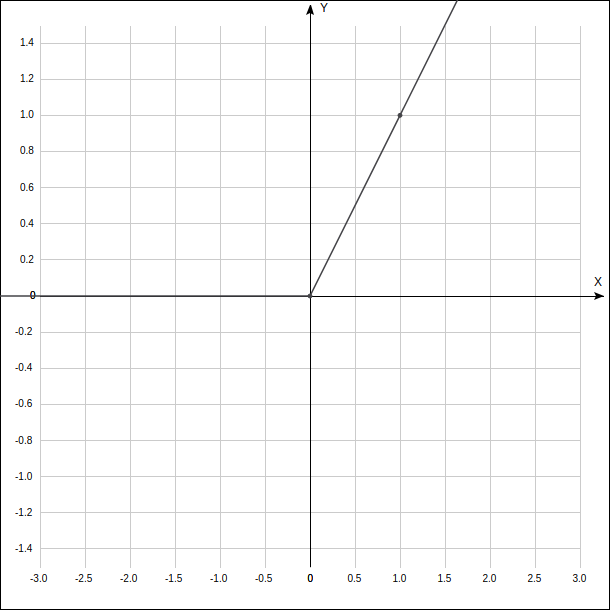
\includegraphics[width=0.5\textwidth]{inc/img/relu.png}
%			\caption{График ReLU}
%			\label{anal:relu}
%		\end{figure}
		
	\end{itemize}
	\item Выходное значение, которое находится по формуле:
	
	\begin{equation}
	a = \sigma( \sum_{i=1}^{n}w_ix_i + b )
	\end{equation}
	
\end{itemize}

Поскольку каждый узел содержит нелинейную функцию, сеть способна изучать различные нелинейные представления входных данных с помощью различных комбинаций входных узлов и функций активации.

\subsubsection{Глубинные нейронные сети}

Глубинные нейронные сети (англ. Deep neural networks) -- нейронные сети с более чем одним скрытым слоем (рис. \ref{anal:DNN}).

\begin{figure}
	\centering
	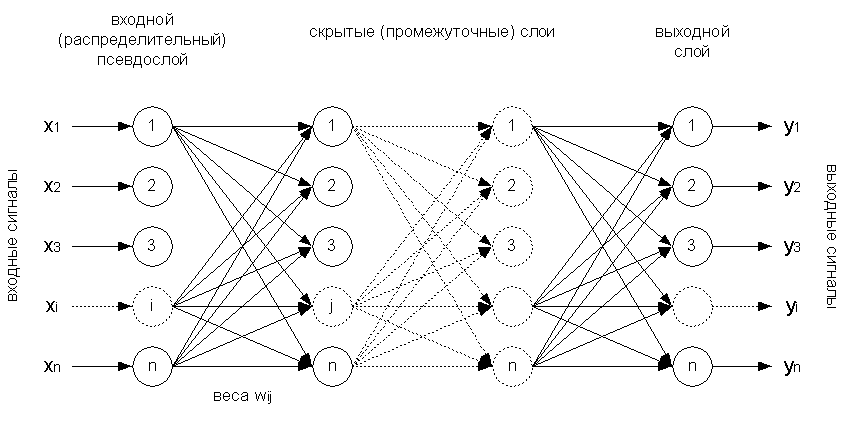
\includegraphics[width=0.8\textwidth]{inc/img/dnn.png}
	\caption{Общая схема ГНС}
	\label{anal:DNN}
\end{figure}

По мере того как данные проходят через более чем один слой, можно обнаружить более абстрактные представления данных, что может помочь улучшить классификацию данных. Каждый слой глубинной сети имеет входы и выходы, и Количество входов каждого слоя зависит от количества выходов его предшественника. Если вход $k-го$ слоя -- $x_k$, то его выход можно записать как:

\begin{equation}
a_k = \sigma_k( b_k + \sum_{i=1}^{n} w_{k,i} x_{k,i} )
\end{equation}

На каждом отдельном слое могут быть использованы отдельные активационные функции.

ГНС рассматривались в качестве инструмента в задачах выделения инструментальных аудио источников\cite{Uhlich}.

Метод состоит из трех основных шагов:

\begin{enumerate}
	\item Препроцессинг
	
	Исходный сигнал $y(n)$ преобразуется в его частотное представление с помощью оконного преобразования Фурье, используя прямоугольную оконную функцию. Из этого представления строится вектор $x \in \Re^{(2C+1)L}$, состоящий из суммы значений магнитуды текущего кадра и $C$ предыдущих/следующих кадров, $L$ -- количество значений магнитуды на кадр.
	
	Полученный вектор нормализуется с помощью числа $\gamma > 0$, являющегося средней Евклидовой нормой $2C+1$ кадоров.
	
	\item Работа глубокой нейронной сети
	
	Полученный нормализованный вектор подается на вход DNN, состоящей из $K$ слоев, с выпрямленной линейной функцией активации (англ. rectified linear unit, ReLU), имеющей вид
	\begin{equation}
	x_{k+1} = max(W_k x_k + b_k , 0), k = 1, ..., K
	\label{anal:relu}
	\end{equation}
	где 
	\begin{itemize}
		\item $x_k$ -- входой вектор для k-го слоя, в частности $x_1$ является исходных вектором, $x_{K+1}$ -- результирующий вектор работы ГНС $\hat s$
		\item $W_k$ -- веса k-го слоя
		\item $b_k$ -- пороговые значения k-го слоя
	\end{itemize}

	Результатом работы ГНС является вектор $\hat s$, являющийся значением магнитудного окна $s \in \Re^L$ выделяемого инструмента.
	
	\item Восстановление
	
	Данный шаг предполагает получение результата применения ОПФ к выделяемому сигналу $s(n)$ при помощи фазы ОПФ исходного сигнала и произведения каждого полученного вектора $\hat{s}$ с коэффициентом нормализации $\gamma$, используемым выше. Получение итогового сигнала происходит с помощью обратного ОПФ.
	
\end{enumerate}

Общая схема работы метода представлена на рисунке \ref{anal:DNN-inst}.

\begin{figure}
	\centering
	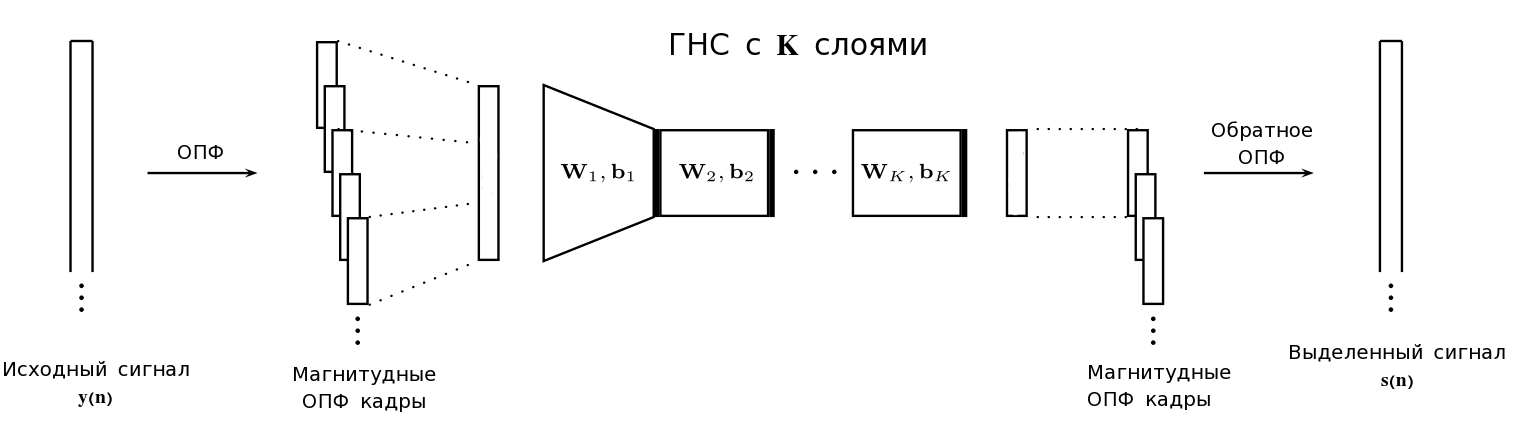
\includegraphics[width=\textwidth]{inc/img/DNN-inst.png}
	\caption{Схема работы метода выделения инструментальных аудио сигналов с использованием ГНС}
	\label{anal:DNN-inst}
\end{figure}

\subsubsection{Сверточные нейронные сети}

Сверточные нейронные сети (англ. Convolutional neural networks) -- это вариант нейронных сетей, вдохновленных зрительной корой головного мозга человека\cite{Hubel}, используются в основном для обработки изображений. СНС используют локальную пространственную корреляцию между входными нейронами из изображения с помощью локальных сенсорных полей. Для иллюстративных целей входной слой вместо одномерного слоя нейронов можно рассматривать как двумерную матрицу, как в случае с файлом изображения. Для изображений значения этой двумерной матрицы представляют интенсивности пикселей. 

В обычной нейронной сети каждый входной нейрон был бы связан с каждый нейроном на первом скрытом слое, в то время как в СНС каждый нейрон первого скрытого слоя связан только с небольшой группой нейронов (рис. \ref{anal:CNN-first}). Сенсорное поле перемещается по всему входному массиву для формирования скрытого слоя. Движение может иметь различный шаг, например на рисунке \ref{anal:CNN-first} изображен шаг (1, 1). Количество нейронов в скрытом слое зависит от количества единиц во входном слое, шага и размера поля.

\begin{figure}
	\centering
	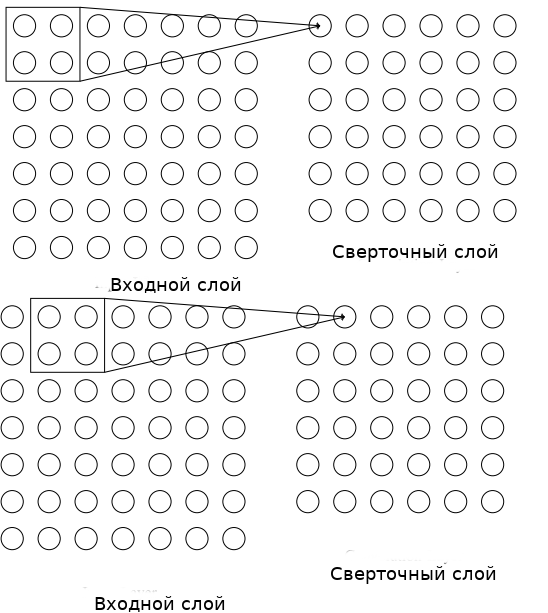
\includegraphics[width=0.6\textwidth]{inc/img/cnn-first.png}
	\caption{Связывание входного слоя с первым скрытым слоем}
	\label{anal:CNN-first}
\end{figure}

Если входной слой имеет размерность $M \times N$, шаг равен (1, 1) и сенсорное поле имеет размерность $A \times B$, то скрытый слой будет иметь размерность $(M - A + 1) \times (N - B + 1)$. Ключевая особенность СНС заключается в том, что нейроны скрытого сверточного слоя разделяют веса и смещения, так что процесс работы сети похож на свертку матрицы размерности $A \times B$ над матрицей $M\times N$.

Результат $j,k-го$ нейрона сверточного слоя математически можно описать как:

\begin{equation}
a_{j,k} = \sigma \Bigg(b + \sum_{l=0}^{A-1} \sum_{m=0}^{B-1} w_{i,m}x_{j+l,k+m}\Bigg)
\end{equation}

Другими словами, сверточный слой вычисляет активацию объекта размерности AxB в разных областях входного слоя. Сопоставление входного слоя с сверточным часто называют векторной картой, а общие веса и единицы смещения называются ядром. Так как каждое из этих ядер идентифицирует одну особенность во входном слое, то сверточный слой обычно включает в себя более одного ядра или карты признаков.

В контексте задачи разделения источников СНС используют для реализации основной идеи ФНМ. В то время, как ФНМ алгоритму необходимо находить базисные вектора для каждой ноты аудиоисточника, рассматриваемый алгоритм использует СНС с целью унификации этих действий через вычесление меньших устойчивых тембральных структур на меньших частях спектограммы. Общая схема работы алгоритма представлена на рисунке \ref{anal:CNN}.

\begin{figure}
	\centering
	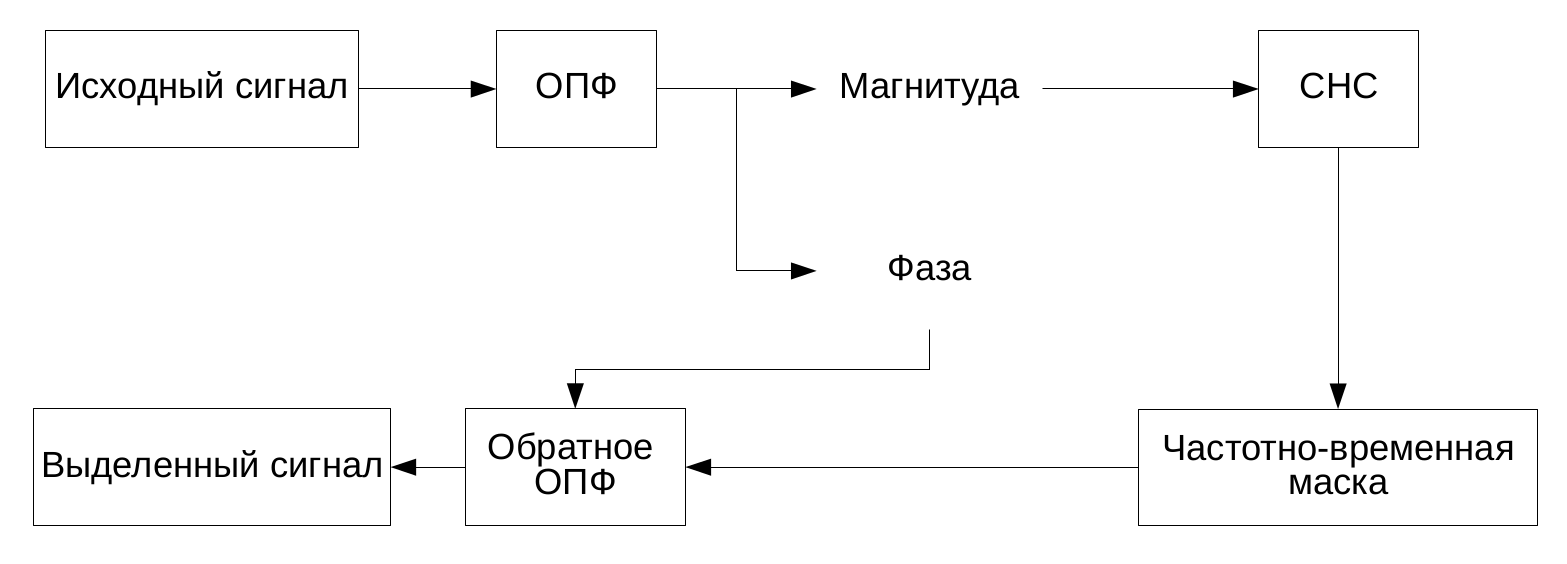
\includegraphics[width=\textwidth]{inc/img/CNN}
	\caption{Схема работы метода выделения аудио сигналов источников с использованием СНС}
	\label{anal:CNN}
\end{figure}

На вход СНС подается магнитудная спектограма, являющаяся результатом применения ОПФ к исходному сигналу. 

Работа нейронной сети происходит в четыре этапа:

\begin{enumerate}
	\item Свертка
	
	Состоит из двух сверточных слоев и объединяющего слоя. 
	\begin{enumerate}
		\item Тембральный сверточный слой: получает локальную информацию о тембре, позволяя модели изучать особенности тембра. В отличие от подхода ФНМ, когда для каждого источника определяются конкретные базисные и активационные вектора, эти характеристики являются общими для отдельных источников.
		\item Объединяющий слой: сжимает информацию, указанную в первом слое по частоте и времени для достижения компактного представления данных. На данном слое сравниваются результаты трех типов: без уплотнения, с уплотнением по частоте и с уплотнением по частоте и времени одновременно.
		\item Временный сверточный слой: изучает различные типы временных изменений для разных инструментов на основании характеристик, полученных из тембрального сверточного слоя. Результатом являются частотно-временные характеристики различных аудио источников. 
	\end{enumerate}
	
	\item Сокращение размерности
	
	Данный слой состоит из нелинейной комбинации признаков, полученных из предыдущих слоев, с ReLU. Слой выбирается таким образом, чтобы иметь меньше элементов для уменьшения общих параметров сети и обеспечения того, чтобы сеть не перегружала данные и могла создавать надежное представление данных.
	
	\item Обратная свертка
	
	Проводятся действия, являющихся обратными операции свертки. Состоит из последовательной развертки и масштабирования данных.
	
	\item Частотно временное экранирование
	
	На данном этапе на основе полученных данных вычисляется частотно-временная маска для каждого выделяемого источника:
	
	\begin{equation}
	m_a t (f) = \frac{|\hat{y}_{at}(f)|}{\sum_{n=1}^{N} |\hat{y}_{nt}(f)|}
	\end{equation}
	
	где $\hat{y}_{nt}(f)$ -- результат работы СНС для $n$-го источника в момент времени $t$, N - число выделяемый источников.
	
	Полученная маска применяется к исходному сигналу, в результате получая спектрограмму выделяемого сигнала:
	\begin{equation}
	y_n(f) = m_n t(f)x_t(f)
	\end{equation}
	
	где $x_t(f)$ -- спектрограмма исходного сигнала.
	
\end{enumerate}

Как и в случае с ГНС, для вычисления выделяемого сигнала, к полученной спектрограмме применяется обратное ОПФ.

\subsubsection{Рекуррентные нейронные сети}

Поскольку аудио сигналы имеют временной контекст, нейронной сети должна быть предоставлена некоторая память для добавления контекстной информации из прошлого. Одним из решений является использование рекуррентной нейронной сети. Суть заключается в соединении скрытого слоя с самим собой (рисунок \ref{anal:rnn}). То есть вход слоя в момент времени t можно описать так:

\begin{equation}
J(j,t) = \sum X(i,t) W_1(i,j) + b_1 W_1(i+1, j) + W_2 H( J(j, t-1) )
\end{equation}

где $H(J(j,t-1))$ -- выход слоя в момент времени $t-1$. 

\begin{figure}
	\centering
	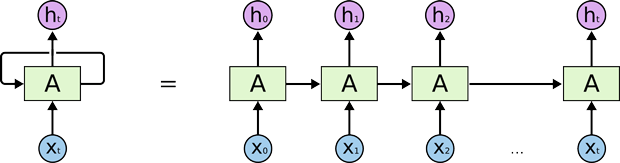
\includegraphics[width=\textwidth]{inc/img/rnn-simple.png}
	\caption{Схема однойслойной рекуррентной нейронной сети}
	\label{anal:rnn}
\end{figure}

Существуют так же многослойные рекуррентные сети. Различают многослойные РНС с одной рекуррентной связью на l-слое и сложенные многослойные РНС, с рекуррентными связями на каждом скрытом слое (рисунок \ref{anal:drnn}).

\begin{figure}
	\centering
	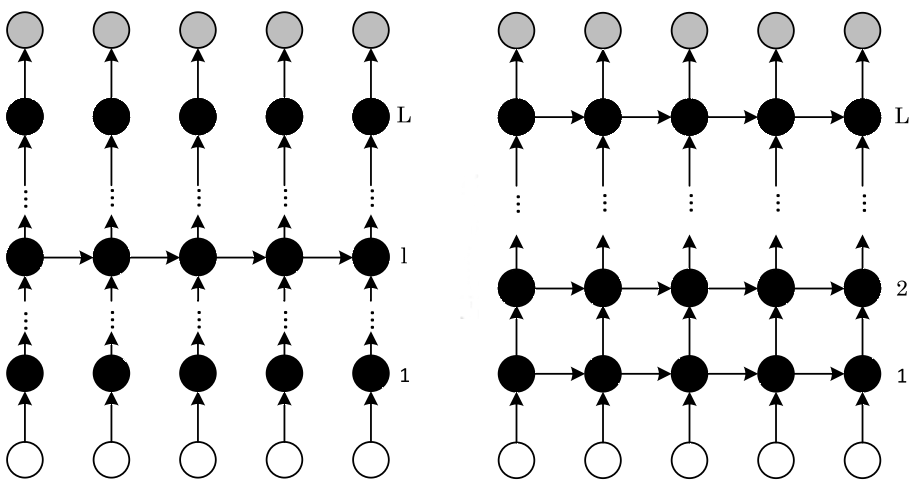
\includegraphics[width=\textwidth]{inc/img/rdnn.png}
	\caption{Схемы многослойной РНС с одной рекуррентной связью и сложенной многослойной РНС, с L скрытыми слоями}
	\label{anal:drnn}
\end{figure}

Эта работа будет сфокусирована на использовании сложенной многослойной РНС. На вход сети будет подаваться спектрограмма исходного сигнала, полученная из ОПФ. Сеть должна генерировать частотно-временную маску, которая на последнем слое будет применяться к спектрограмме исходного слоя.

\section{Оценка методов выделения источников}

Оценка методов выделения источников является нетривиальной задачей, учитывая субъективность мнения о качестве аудио записи. Тем не менее, оценочные метрики были изучены и формализованы группой исследователей во главе с Имануилом Винсентом\cite{Vincent}.
Оценка метода выделения аудио источника должна проходить в контексте приложения. Исходный сигнал представляется линейной комбинацией сигналов источников $(s_j)_{j\in J}$ с добавлением шума. Простейшей мерой является норма L2, выражающаяся в разнице между полученным источником $\hat{s}_j$ и ожидаемым источником $s_j$:

\begin{equation}
D = \min_{\epsilon=\pm 1} \Bigg | \Bigg | \frac{\hat{s}_j}{||\hat{s}_j||} - \epsilon \frac{s_j}{||s_j||} \Bigg | \Bigg |^2
\end{equation}

Данная разность всегда неотрицательна и равна нулю только в случае $\hat{s}_j = s_j$. В худшем случае, когда вектора $\hat{s}_j$ и $\hat{s}$ ортогональны, разность останется ограниченной максимумом двух, так как источники нормализованы. Так же, в случае шумов или других искажений, которые добавляются к искомым источниками, данная мера будет имет низкое значение, которое может быть нежелательным, в зависимости от приложения. Например, при обработке аудиозаписей высокого качества, такие шумы могут быть нежелательными, а в случае, когда к выделяемым источникам планируется применять дополнительную, данными искажениями можно пренебречь.

Для учета этих случаем искомый источник разделяется на четыре части:

\begin{equation}
\hat{s}_j = s_{target} + e_{interf} + e_{spat} + e_{artif}
\label{anal:source}
\end{equation}

где

\begin{itemize}
	\item $s_{targer}$ -- модификация целевого источника, которая может содержать определенные допустимые искажения, $F$;
	\item $e_{interf}$ -- помехи, полученные от нежелательных источников $(s_{j'})_{j' \neq j}$;
	\item $e_{spat}$ -- пространственные искажения;
	\item $e_{artif}$ -- остальные виды шумов, не входящие в $F$ и другие артефакты.
\end{itemize}

Для определения метрик используются ортогональные проекции, которые могут быть определены следующим образом: для подпространства с векторами $y_1, y_2, ... , y_n$, $\prod{y_1, y_2, ... , y_n}$ -- матрица, проектирующая вектора в данное подпространство. Определяются следующие матрицы:

\begin{equation}
P_{s,j} = \prod(s_j)
\end{equation}

\begin{equation}
P_{S} = \prod\{(s_{j'})_{1\le j' \le n}\}
\end{equation}

\begin{equation}
P_{S, n} = \prod\{(s_{j'})_{1\le j' \le n}, (n_i)_{1 \le i \le m} \}
\end{equation}

С помощью этих проецирующих матриц слагаемые из формулы \ref{anal:source} можно представить следующим образом:

\begin{equation}
	s_{target} = P_{s,j} \hat{s}_j
\end{equation}

\begin{equation}
e_{interf} = P_{S} \hat{s}_j - P_{s,j} \hat{s}_j
\end{equation}

\begin{equation}
e_{spat} = P_{S, n} \hat{s}_j - P_{s,j} \hat{s}_j
\end{equation}

\begin{equation}
e_{artif} = \hat{s}_j - P_{S, n} \hat{s}_j
\end{equation}

Для вычисления $s_{target}$ используется скалярное произведение:

\begin{equation}
s_{target} = (\hat{s}_j, s_j) \frac{s_j}{|| s_j ||^2}
\end{equation}

Для вычесления $P_S$ и $P_{S,n}$ используется вектор коэффициентов $c$:

\begin{equation}
c = R_{SS}^{-1}[ (\hat{s}_j, s_1) ... (\hat{s}_j, s_n) ]^H
\end{equation}

где $R_{SS}$ -- определитель Грама (грамиан). $P_S \hat{s}_j$ можно записать как:

\begin{equation}
P_S \hat{s}_j = c^H s
\end{equation}

где $(.)^H$ -- Эрмитовская перестановка. 

Если источник и шумовой сигнал взаимно ортогональны, то можно записать:

\begin{equation}
	e_{interf} = \sum_{j' \ne j} (\hat{s}_j, s_{j'}) \frac{s_{j'}}{|| s_{j'} ||^2}
\end{equation}

\begin{equation}
P_{S,n}\hat{s}_j = P_S \hat{s}_j + \sum_{i=1}^{m}(\hat{s}_j, n_i) \frac{n_i}{|| n_i ||^2}
\end{equation}

На основании этих значений можно записать следующие метрики:

\begin{enumerate}
	\item Отношение источника к искажению:
	
	\begin{equation}
		SDR = 10 \log_{10} \frac{|| s_{target} ||^2}{|| e_{interf} + e_{spat} + e_{artif} ||^2}
	\end{equation}
	
	Эта мера оценивает общую эффективность алгоритма разделения источников
	
	\item  Отношение источника к интерференции:
	
	\begin{equation}
		SIR = 10 \log_{10} \frac{|| s_{target} ||^2}{|| e_{interf} ||^2}
	\end{equation}
	
	Эта мера отражает подавление помех во время выделения.
	
	\item Отношение образа к пространственному искажению:
	
	\begin{equation}
	ISR = 10 \log_{10} \frac{|| s_{target} + e_{interf} ||^2}{|| e_{spat} ||^2}
	\end{equation}
	
	\item Отношение источника к артефактам:
	
	\begin{equation}
	SAR = 10 \log_{10} \frac{|| s_{target} + e_{interf} + e_{spat} ||^2}{|| e_{artif} ||^2}
	\end{equation}
	
	Эта мера оценивает артефакты, получаемые во время разделения источников.
\end{enumerate}

Значение компонент $s_{target}, e_{interf}, e_{spat}$ и $e_{artif}$ изменяются во времени. Предлагается разделять сигнал на части для вычисления локальных значений. Итоговые значения могут быть суммированы с использованием статистических мер.

\section{Сравнение методов}

Метод главных компонент и Факторизация неотрицательных матриц не участвуют в сравнении, так как являются строго статистическими методами и требуют дополнительных действий для подбора начальных значений для каждого конкретного примера.

\begin{table}[h]
	\caption{\label{tab:canonsummary}Сравнение алгоритмов выделения источников}
	\begin{center}
		\begin{tabular}{|c|c|c|c|}
			\hline
			Метод & Метрика & Вокал & Аккомпанемент \\
			\hline
			CNN & SDR & -0.6 ± 4.9 & 4.5 ± 1.2 \\
				& SIR & 1.9 ± 6.2 & 14.9 ± 5.6 \\
				& SAR & 3.6 ± 2.1 & 16.4 ± 2.9 \\
				& ISR & 7.3 ± 2.7 & 6.9 ± 1.0 \\
			\hline
			DNN & SDR & -8.9 ± 4.4 & 4.1 ± 2.6 \\
			& SIR & 10.8 ± 3.1 & 10.7 ± 3.8 \\
			& SAR & -6.6 ± 4.6 & 12.1 ± 3.9 \\
			& ISR & 4.8 ± 2.8 & 5.0 ± 3.0 \\
			\hline
			FASST & SDR & -1.8 ± 5.8 & 8.9 ± 3.2 \\
			& SIR & -3.7 ± 7.5 & 13.7 ± 3.0 \\
			& SAR & 4.3 ± 1.4 & 13.1 ± 3.2 \\
			& ISR & 5.6 ± 2.5 & 13.5 ± 2.5 \\
			\hline
		\end{tabular}
	\end{center}
\end{table} 

Значение метрик получено на наборе данных DSD100 \cite{DSD100}. Как видно из таблицы, использование нейронных сетей дает лучший результат в задаче выделения аудио источников.

\section{Вывод}

Необходимо разработать и реализовать метод выделения голосовой составляющей из монофонического аудио сигнала на основе многослойной РНС.

Для выполнения работы необходимо спроектировать и реализовать продукт, осуществляющий автоматизированное выделение вокальной составляющей из музыкального аудио сигнала. На вход программному продукту подаются одноканальные музыкальные произведения в формате WAVE. На выходе программный продукт генерирует два одноканальных WAVE-файла, содержащие вокальный аудио сигнал и аккомпанемент. Исходные музыкальные произведения должны представлять из себя песни с эстрадным стилем вокала. Разделяемые записи должны представлять собой записи <<без потерь>>, на них не должно быть шумов. Для более точного разделения запись должна быть без фильтров, применяемых на этапе пост-обработки.

Для определения качества выделения источников будут использоваться сравнение полученных в результате работы алгоритмов данных с заранее известными на основе описанных выше метрик.

Так же необходимо сравнить показатели разработанного метода с значениями, описанными в таблице \ref{tab:canonsummary}.

%%% Local Variables:
%%% mode: latex
%%% TeX-master: "rpz"
%%% End:

\chapter{Конструкторский раздел}
\label{cha:design}

\section{Архитектура программного продукта}

Разрабатываемый программный продукт состоит из следующих частей:

\begin{enumerate}
	\item модуль обработки входных данных;
	\item модуль генерации магнитуд для вокала и аккомпанемента;
	\item модуль формирования выходных данных.
\end{enumerate}

IDEF0 диаграмма программы показаны на рисунке \ref{des:idef0}.

\begin{figure}
	\centering
	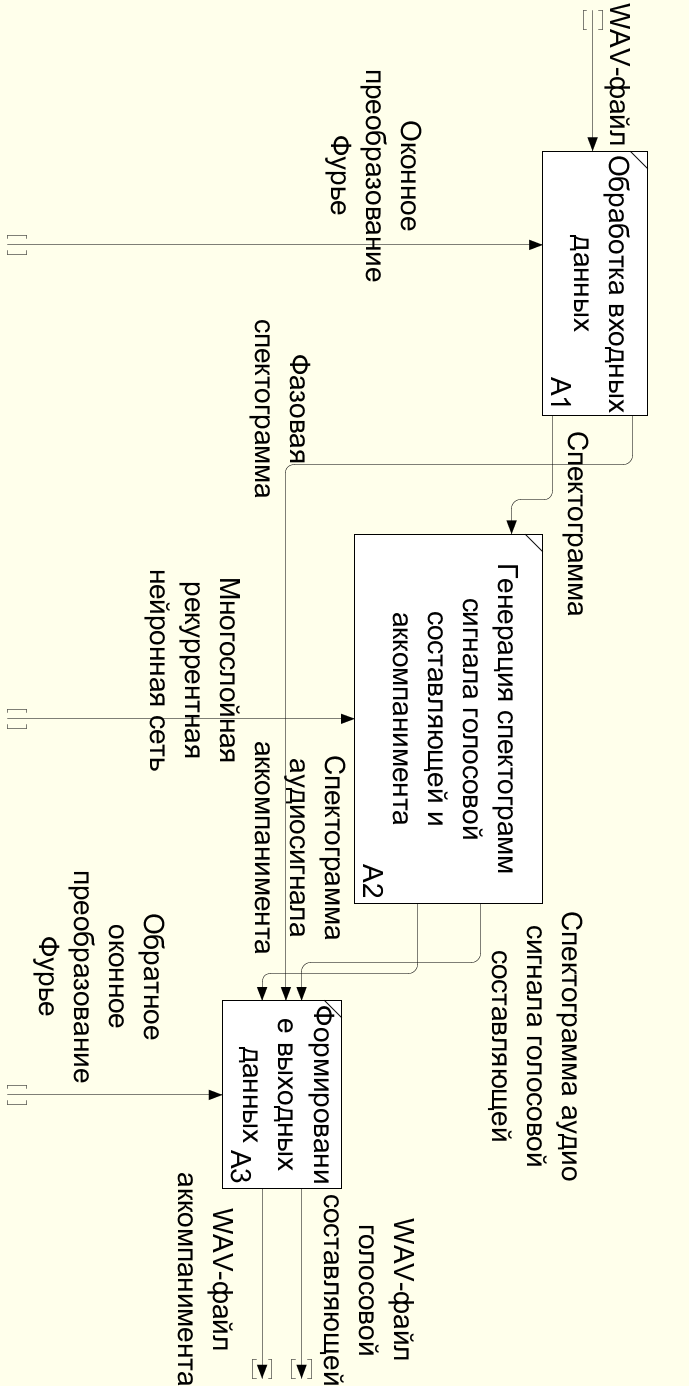
\includegraphics[width=0.6\textwidth]{inc/img/idef}
	\caption{IDEF0 программного продукта}
	\label{des:idef0}
\end{figure}

\section{Алгоритмы}

Алгоритм \ref{des:pseudo} описывает процесс выделения вокальной составляющей из аудио сигнала. Подробное описание представлено ниже.

\begin{algorithm}[H]
	\label{des:pseudo}
	\SetAlgoLined
	\KwIn{Аудио сигнал $x(t)$}
	\KwOut{Аудио сигнал голосовой составляющей $y_1(t)$, аудио сигнал аккомпанимента $y_2(t)$}
	\KwData{Оконная функция $w$}
	
	Получение спектрограммы с помощью ОПФ:
	
	$s(f, n) \leftarrow$ ОПФ($x(t), w$)
		
	Получение амплитудной и фазовой характеристик спектограммы:
	
	$m(f, n) \leftarrow | s(f,n)|$
	
	$p(f, n) \leftarrow andle(s(f,n))$
	
	Получение амплитудных характеристик спектрограмм выделяемых источников:
	
	$\tilde{y_1}(f, n), \tilde{y_2}(f, n) \leftarrow DRNN(m(f, n))$
	
	Получение сигналов выделяемых источников с помощью обратного ОПФ:
	
	$ y_1(t), \leftarrow $ ООПФ $(\tilde{y_1}(f, n), p(f, n))$
	
	$ y_2(t), \leftarrow $ ООПФ $(\tilde{y_2}(f, n), p(f, n))$
	\caption{Алгоритм выделения аудио источников}
\end{algorithm}

\subsection{Обработка входных данных}

Чтение аудио-файлов, хранящиеся в формате WAVE, происходит с помощью библиотеки. Результатом работы библиотечной функции является информация о частоте дискретизации и структура со значениями амплитуд сигнала. 

После считывания аудио-файла происходит построение его спектра при помощи оконного преобразования Фурье. Результатом работы этого алгоритма является структура, в которой хранятся наборы частот по отрезкам времени.

В качестве оконной функции используется Окно Ханна, дискретная функция которого которого записывается следующим образом:

\begin{equation}
w(n) = 0.5 - 0.5 \cos \Big(\frac{2\pi n}{N-1}\Big)
\end{equation}

\subsection{Генерация частотно-временных масок}

Для получения частотно-временных масок используется многослойная рекуррентная нейронная сеть. На ее вход подается результат применения ОПФ к исходному сигналу. Результатом работы сети являются спектрограммы выделяемых источников.

\subsection{Описание сети}
Многослойная РНС состоит из 6 слоев:

\begin{enumerate}
	\item Входной слой. На вход подается спектрограмма исходного сигнала, полученная в следствии применения ОПФ.
	\item 3 скрытых слоя $h_t^1, h_t^2$ и $h_t^3$. 
	
	Слой $h_t^2$ имеет рекуррентную связь. Отсюда результатом работы этого слоя в момент времени $t$ можно записать как:
	
	\begin{equation}
	h_t^2 = f_h(x_t, h_{t-1}^2) = \sigma_2 (U^2 h_{t-1}^2 + W^2(h_{t}^1))
	\end{equation}
	
	где:
	
	\begin{itemize}
		\item $W^i$ -- веса связей, идущих от предшествующего слоя;
		\item $U^i$ -- веса рекуррентной связи;
		\item $h_t^{i-1}$ -- результат работы предшествующего слоя;
		\item $\sigma_i$ -- активационная функция.
	\end{itemize}

	Так как у первого слоя предшествующий слой -- входной, то его результат вычисляется по следующей формуле:
	
	\begin{equation}
	h_t^1 = \sigma_1 ( W^1 x_t)
	\end{equation}
	
	Результатом работы слоя $h_t^3$ будет:
	
	\begin{equation}
	h_t^3 = \sigma_3 (W^2 h_t^2)
	\end{equation}
	
	В качестве активационной функции используется ReLU (формула \ref{anal:relu}).
	
	\item Слой генерации частотно-временных масок. Данный слой использует результат работы слоя третьего рекуррентного слоя для генерации двух векторов $\hat{y}_{1t}$ и $\hat{y}_{2t}$, размер которых равен размеру входного вектора. Данные последовательности используются для вычисления частотно-временной маски $m_t(f)$, которая является функцией частоты:
	
	\begin{equation}
	m_t(f) = \frac{|\hat{y}_{1t}(f)|}{|\hat{y}_{1t}(f)| + |\hat{y}_{1t}(f)|}
	\label{des:mask}
	\end{equation}
	
	\item Слой генерации спектрограмм. Для получение спектрограмм выделяемых источников к спектрограмме исходного аудио-сигнала применяется частотно-временная маска, полученная на предыдущем слое. В итоге получаются два вектора $\tilde{y}_{1t}$ и $\tilde{y}_{2t}$, вычисляющиемся как:
	
	\begin{equation}
	\tilde{y}_{1t}(f) = m(f)x_t(f)
	\end{equation}
	
	
	\begin{equation}
	\tilde{y}_{2t}(f) = (1 - m(f))x_t(f)
	\end{equation}
	
	С учетом формулы \ref{des:mask}:
	
	\begin{equation}
	\tilde{y}_{1t} = \frac{|\hat{y}_{1t}|}{|\hat{y}_{1t}| + |\hat{y}_{1t}|} \bigodot x_t
	\end{equation}
	
	
	\begin{equation}
	\tilde{y}_{2t} = \frac{|\hat{y}_{2t}|}{|\hat{y}_{1t}| + |\hat{y}_{1t}|} \bigodot x_t
	\end{equation}
	
\end{enumerate}

\begin{figure}
	\centering
	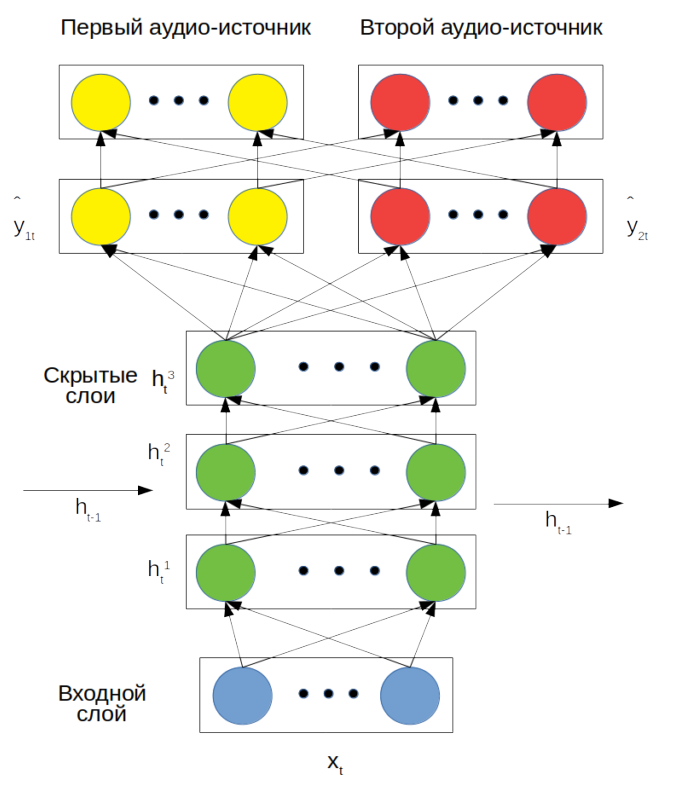
\includegraphics[width=\textwidth]{inc/img/drnn-design}
	\caption{Схема нейронной сети}
	\label{des:drnn}
\end{figure}


Схема нейронной сети представлена на рисунке \ref{des:drnn}.

\subsubsection{Обучение нейронной сети}

Для обучения нейронной сети используется Метод обратного распространения ошибки. Для вычисления ошибок между сгенерированными векторами $ \tilde{y}_{1t}, \tilde{y}_{2t} $ и ожидаемыми $ y_{1t}, y_{2t} $ используются среднеквадратичное отклонение

\begin{equation}
J_{MSE} = || \tilde{y}_{1t} - y_{1t} ||^2 + || \tilde{y}_{2t} - y_{2t} ||^2
\end{equation}

и дивергенция Кулбека-Лейблера

\begin{equation}
J_{KL} = D(y_{1t}, \tilde{y}_{1t}) + D(y_{2t}, \tilde{y}_{2t})
\end{equation}

где $D$ вычисляется по формуле \ref{anal:kl}.

\subsection{Формирование выходных данных}

Для формирования WAV-файлов используется обратное оконное преобразование Фурье. В качестве параметров передается матрица, полученная из спектрограммы выделяемого источника и фазовой спектрограммы исходного сигнала.

\section{Используемые структуры данных}

Для хранения данных WAV-файла используется последовательность действительных чисел, хранящая информацию об уровне сигнала в определенным момент времени.

Для хранения результатов ОПФ и работы нейронной сети используется матрица комплексных чисел, так как требуется быстрый доступ к элементам, а изменений размеров после первичного заполнения не происходит. 

Комплексное число представляет собой структуру с двумя полями: реальной и мнимой частями.

В качестве входных данных нейронной сети используется используется амплитудная характеристика спектрограммы, хранящаяся в виде матрицы действительных чисел фиксированного размера.

\section{Тестирование}

Тестирование программного продукта заключается в сравнении результата работы методов на тестовых наборах данных с заранее заданным результатом. Тестовые наборы данных (англ. dataset) для проверки работы алгоритмов, связанных с обработкой музыкальных произведений, предоставляются в открытом доступе в Интернете.

Важной характеристикой входных данных является стиль вокала, так как разные стили имеют разные спектральные характеристики. Можно выделить следующие классы эквивалентности:

\begin{itemize}
	\item академический вокал(классический, оперный);
	\item эстрадный вокал;
	\item джазовый вокал;
	\item рок вокал;
	\item народное пение;
	\item горловое пение.
\end{itemize}

Следует протестировать работу алгоритмов на музыкальных произведениях с эстрадным вокалом.

\subsection{Тестовые данные}

Для тестирования программного продукта используется открытый набор данных DSD100 (Community-Based Signal Separation Evaluation Campaign 2016). В DSD100 содержатся 100 музыкальных произведений разных жанров, с мужским и женским вокалом. Каждый музыкальный трек был сведен с использованием профессиональных средств звукозаписи.

DSD100 состоит из WAV-файлов сведенных музыкальных произведений, хранящихся в папке <<Mixture>>, и WAV-файлов источников, хранящихся в папке <<Sources>>.

Источники разделены на 4 типа:

\begin{itemize}
	\item вокал;
	\item бас;
	\item ударные;
	\item остальное.
\end{itemize}

Все записи являются полифоническими (двух-канальными).

Для тестирования разработанного метода данный датасет необходимо привести к следующему виду. Все источники приводятся в монофонический формат. Бас, ударные и остальное объединяются в один WAV-файл.

\section{Вывод}

В конструкторском разделе описывается предлагаемый метод выделения голосовой составляющей из монофонического аудио сигнала. Дано подробное описание, построены схемы выбранных алгоритмов. При этом выделены основные этапы работы метода с указанием необходимых исходных данных для его работы и полученных результатов на каждом этапе

%%% Local Variables:
%%% mode: latex
%%% TeX-master: "rpz"
%%% End:

%\chapter{Технологический раздел}
\label{cha:impl}

В данном разделе описываются средства, используемые для разработки программного продукта, требования для функционирования ПО, описываются результаты тестирования программного продукта.

\section{Выбор средств разработки}

\subsection{Выбор языка программирования}

Для написания программного продукта используется язык Python, так как для него существует множество готовых решений для работы с нейронными сетями. Так же выбранный язык сочетает в себе возможности функционального, структурного и объектно-ориентированного подходов, что позволяет кратко описывать математические конструкции, необходимые для решения поставленной задачи. Так же для данного языка существует большое количество различных математических библиотек, упрощающие работу с комплексными числами, и библиотек для обработки цифровых сигналов.

\subsection{Выбор среды программирования и отладки}

В качестве среды разработки для языка Python была выбрана кроссплатформенная IDE PyCharm. Предоставляет средства для анализа кода, графический отладчик, инструмент для запуска юнит-тестов. На данный момент PyCharm является бесплатным для образовательных учреждений и проектов с открытым исходным кодом.

Выбор данной среды разработки обусловлен следующими предоставляемыми возможностями, упрощающими разработку приложения и способствующими повышению качества исходного кода:

\begin{itemize}
	\item статический анализ кода;
	\item встроенный отладчик;
	\item навигация по проекту и исходному коду;
	\item рефакторинг;
	\item поддержка систем контроля версий.
\end{itemize}

\subsection{Используемые библиотеки}

Для упрощения реализации математических операций используется библиотека NumPy. Для считывания и записи аудио-файлов, а так же обработки сигналов используется библиотека LibROSA. Для работы с нейронной сетью используется библиотека TensorFlow. Для создания интерфейса используется фреймворк PyQt, который является Python-версией C++ фреймворка Qt.

\section{Система контроля версий}

В процессе разработки программы использовалась система контроля версий
Git. Система контроля версий позволяет вносить в проект атомарные изменения, направленные на решения каких-либо задач. В случае обнаружения ошибок или из- менения требований, вне-сенные изменения можно отменить. Кроме того, с помощью системы контроля версий решается вопрос резервного копирования.

Особенности Git:

\begin{itemize}
	\item данная система контроля версий является децентрализованной, что позволяет иметь несколько независимых резервных копий проекта;
	\item поддерживается хостингом репозиториев GitLab;
	\item поддерживается средой разработки PyCharm;
	\item предоставляет широкие возможности для управления изменениями проекта и просмотра истории изменений.
\end{itemize}

\section{Требования к вычислительной системе}

Для запуска программы необходимо иметь установленный на ЭВМ интерпретатор для Python 3.6 с установленными библиотеками. 

Так как выбранный язык программирования является кроссплатформенным, то требований к использованию операционной системы нет.

Алгоритмы работают с большими объёмами комплексных данных, поэтому объём оперативной памяти компьютера не должен быть меньше 1 ГБ, желательна архитектура x64 (x86-64).

\section{Формат данных}

Входом и выходом программного продукта являются WAV-файлы. Формат WAVE имеет четкую структуру, описанную в \cite{wav}.

WAV -- формат файла-контейнера для хранения записи оцифрованного аудиопотока, в котором для кодирования амплитуды вы- деляется фиксированное число бит.

WAV-файл состоит из двух частей. Одна из них -- заголовок файла, другая -- область данных. В заголовке файла хранится информация о:

\begin{itemize}
	\item размере файла;
	\item количестве каналов;
	\item частоте дискретизации;
	\item количестве бит в сэмпле (глубине звучания).
\end{itemize}

Длина заголовка составляет 44 байта. Область данных представляет собой набор амплитуд. 

В программе используется информация о количестве каналов и частоте дискретизации, а также амплитуды.

\section{Диаграмма классов}

Разработанный программный комплекс имеет два режима работы: режим обучения и нормальный режим. Диаграммы классов представлены на рисунках \ref{imp:train} и \ref{imp:run-diagram} соответственно.

\begin{figure}
	\centering
	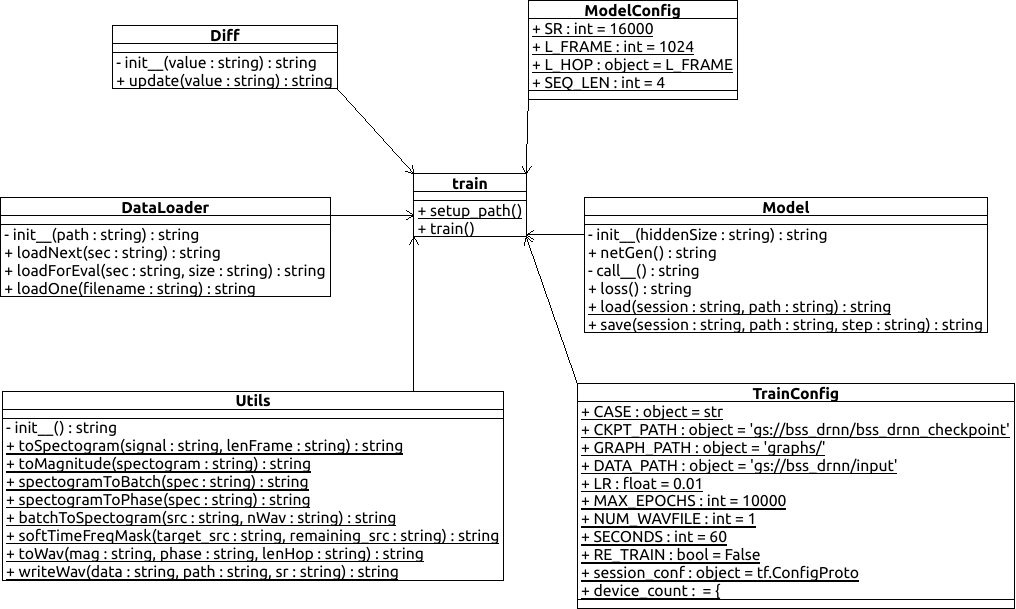
\includegraphics[width=\textwidth]{inc/img/train}
	\caption{Диаграмма классов программы нормального режима}
	\label{imp:train}
\end{figure}

\begin{figure}
	\centering
	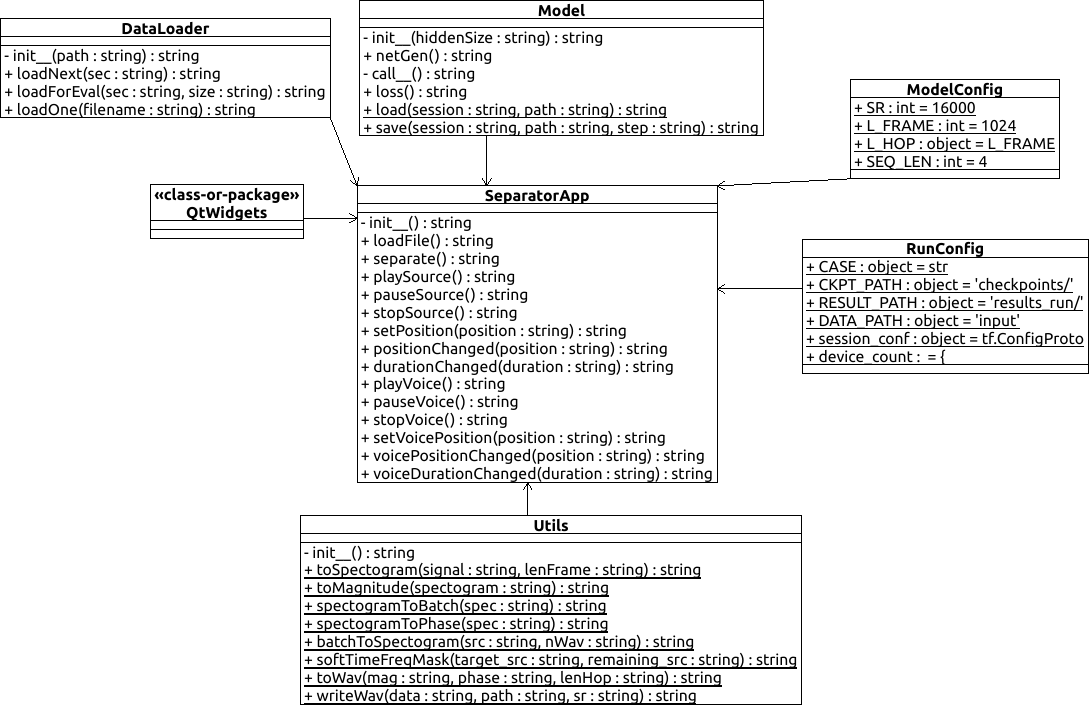
\includegraphics[width=\textwidth]{inc/img/run}
	\caption{Диаграмма классов программы нормального режима}
	\label{imp:run-diagram}
\end{figure}

\subsection{Описание классов}

\subsubsection*{DataLoader}

Отвечает за загрузку wav-файлов. Описание методов представлено в таблице \ref{imp:dataloader}.

\begin{table}[h]
	\caption{\label{imp:dataloader}Описание методов класса DataLoader}
	\begin{center}
		\begin{tabular}{|p{0.45\textwidth}|p{0.45\textwidth}|}
			\hline
			Метод & Описание \\
			\hline
			loadNext(sec) & Считывает очередной wav-файл из тренировочного набора данных, преобразуя его длину в sec \\
			\hline
			loadForEval(sec, size) & Считывает size случайных wav-файлов из тестового набора данных, преобразуя их длину в sec \\
			\hline
			loadOne(filename) & Считывает один файл с именем filename \\ 			
			\hline
		\end{tabular}
	\end{center}
\end{table} 

\subsubsection*{Diff}

Представляет ошибку, получаемую в процессе обучения и ее изменение. Описание методов представлено в таблице \ref{imp:diff}.

\begin{table}[h]
	\caption{\label{imp:diff}Описание методов класса Diff}
	\begin{center}
		\begin{tabular}{|p{0.45\textwidth}|p{0.45\textwidth}|}
			\hline
			Метод & Описание \\
			\hline
			update(sec) & Обновление значения ошибки и вычисление разницы с предыдущей ошибкой \\	
			\hline
		\end{tabular}
	\end{center}
\end{table} 

\subsubsection*{Model}

Представляет модель нейронной сети. Описание методов представлено в таблице \ref{imp:model}.

\begin{table}[h]
	\caption{\label{imp:model}Описание методов класса Model}
	\begin{center}
		\begin{tabular}{|p{0.45\textwidth}|p{0.45\textwidth}|}
			\hline
			Метод & Описание \\
			\hline
			load(session, path) & Загружает информацию об обученной модели для сессии sess из файлов сохранения, расположенных в path \\	
			\hline
			save(session, path) & Сохраняет информацию о модели из сессии sess в папку path \\
			\hline
			netGen() & Генерация нейронной сети \\
			\hline
		\end{tabular}
	\end{center}
\end{table} 

\subsubsection*{ModelConfig}

Представляет класс конфигурации для класса Model. Описание атрибутов представлено в таблице \ref{imp:modelconfig}.

\begin{table}[h]
	\caption{\label{imp:modelconfig}Описание методов класса Model}
	\begin{center}
		\begin{tabular}{|p{0.45\textwidth}|p{0.45\textwidth}|}
			\hline
			Атрибут & Описание \\
			\hline
			SR & Частота дискретизации wav-файла \\	
			\hline
			L\_FRAME & Размер окна в ОПФ \\
			\hline
			L\_HOP & Количество аудио кадров между столбцами ОПФ \\
			\hline
		\end{tabular}
	\end{center}
\end{table}

\subsubsection*{RunConfig}

Представляет класс конфигурации для класса SeparationApp. Описание атрибутов представлено в таблице \ref{imp:runconfig}.

\begin{table}[h]
	\caption{\label{imp:runconfig}Описание атрибутов класса RunConfig}
	\begin{center}
		\begin{tabular}{|p{0.45\textwidth}|p{0.45\textwidth}|}
			\hline
			Атрибут & Описание \\
			\hline
			CKPT\_PATH & Путь к файлам сохранения обученной модели \\	
			\hline
			RESULT\_PATH & Путь сохранения результата работы метода выделения \\
			\hline
			session\_conf & Конфигурация сессии tensorflow \\
			\hline
		\end{tabular}
	\end{center}
\end{table}

\subsubsection*{SeparationApp}

Представляет контроллер работы программы в нормальном режиме. Описание основных методов представлено в таблице \ref{imp:app}.

\begin{table}[h]
	\caption{\label{imp:app}Описание методов класса SeparationApp}
	\begin{center}
		\begin{tabular}{|p{0.45\textwidth}|p{0.45\textwidth}|}
			\hline
			Метод & Описание \\
			\hline
			loadFile() & Загрузка файла с помощью файлового менеджера \\	
			\hline
			separate() & Исполнение метода выделения источников \\
			\hline
		\end{tabular}
	\end{center}
\end{table} 

\subsubsection*{train}

Представляет контроллер работы программы в режиме обучения. Описание основных методов представлено в таблице \ref{imp:train-}.

\begin{table}[h]
	\caption{\label{imp:train-}Описание методов класса train}
	\begin{center}
		\begin{tabular}{|p{0.45\textwidth}|p{0.45\textwidth}|}
			\hline
			Метод & Описание \\
			\hline
			setup\_path() & Настройка путей для файлов сохранения \\	
			\hline
			train() & Обучение нейронной сети \\
			\hline
		\end{tabular}
	\end{center}
\end{table} 

\subsubsection*{TrainConfig}

Представляет класс конфигурации для класса train. Описание атрибутов представлено в таблице \ref{imp:trainconfig}.

\begin{table}[h]
	\caption{\label{imp:trainconfig}Описание атрибутов класса TrainConfig}
	\begin{center}
		\begin{tabular}{|p{0.45\textwidth}|p{0.45\textwidth}|}
			\hline
			Атрибут & Описание \\
			\hline
			CKPT\_PATH & Путь к файлам сохранения обученной модели \\	
			\hline
			GRAPH\_PATH & Путь к файлам сохранения инфографики процесса обучения \\	
			\hline
			DATA\_PATH & Путь к файлам обучающей выборки \\
			\hline
			LR & Коэффициент обучения \\
			\hline
			MAX\_EPOCHS & Количество эпох обучения \\
			\hline
			session\_conf & Конфигурация сессии tensorflow \\
			\hline
		\end{tabular}
	\end{center}
\end{table}

\subsubsection*{Utils}

Представляет вспомогательные функции. Описание методов представлено в таблице \ref{imp:utils}.

\begin{table}[h]
	\caption{\label{imp:utils}Описание методов класса Utils}
	\begin{center}
		\begin{tabular}{|p{0.45\textwidth}|p{0.45\textwidth}|}
			\hline
			Метод & Описание \\
			\hline
			toSpectogram(signal, lenFrame, lenHop) & Получение спектрограммы сигнала \\	
			\hline
			toMagnitude(spectogram) & Амплитудная составляющая спектрограммы \\
			\hline
			spectogramToPhase(spec) & Фазовая составляющая спектрограммы \\
			\hline
			toWav(mag, phase, lenHop) & Преобразование спектрограммы в сигнал \\
			\hline
			writeWav(data, path, sr) & Запись сигнала в аудио файл \\
			\hline
		\end{tabular}
	\end{center}
\end{table} 

\section{Построение нейронной сети}

В представлении Tensorflow нейронная сеть является графом потока данных, в котором данные в виде многомерного массива переходят в разные узлы, в процессе чего происходят все необходимые вычисления.

Каждое вычисление в TensorFlow представляется как граф потока данных. У него есть два элемента:

\begin{itemize}
	\item tf.Operation -- единицы вычислений.
	\item tf.Tensor -- представляет единицы данных (тенсоры).
\end{itemize}

Алгоритм \ref{imp:init-model} описывает инициализацию модели. Для определения входных и выходных данных используются тенсоры типа tf.placeholder. Плейсхолдер нужен исключительно в качестве цели наполнения. Он не инициализирован и не содержит данных.

\begin{minipage}{0.75\textwidth}
\begin{algorithm}[H]
\lstinputlisting[language=Python]{inc/src/model.py}
\caption{Исходный код инициализации модели}
\label{imp:init-model}
\end{algorithm}
\end{minipage}

Алгоритм \ref{imp:gen-model} описывает генерацию сети. Библиотека Tensorflow позволяет описывать граф многослойной рекуррентной нейронной сети с помощью встроенной функций tf.nn.dynamic\_rnn. В качестве параметра в функцию передается объект типа RNNCell.

Для описания графа обычных слоев используется функция tf.layers.dense.

\begin{minipage}{0.75\textwidth}
\begin{algorithm}[H]
	\lstinputlisting[language=Python]{inc/src/gen.py}
	\caption{Исходный код генерации сети}
	\label{imp:gen-model}
\end{algorithm}
\end{minipage}

Итоговый граф изображен на рисунке \ref{imp:graph}.

\begin{figure}
	\centering
	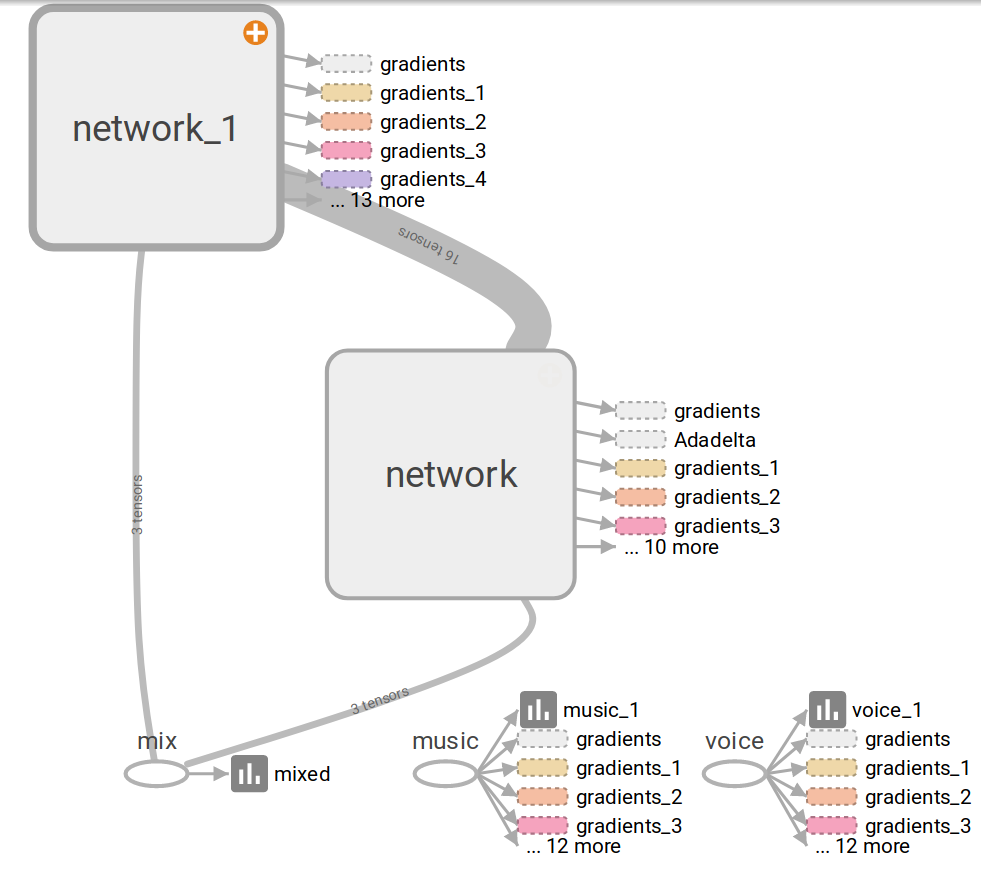
\includegraphics[width=0.7\textwidth]{inc/img/tensorboard-main}
	\caption{Граф модели}
	\label{imp:graph}
\end{figure}

\section{Установка программного обеспечения}

Для работы программного комплекса необходимо иметь на ПК интерпретатор для Python 3, установщик которого поставляется вместе с программным обеспечением. Для установки необходимых библиотек используется каталог программного обеспечения PyPI (Python Package Index). Все необходимые зависимости указаны в файле requirements.txt, благодаря чему установка библиотек выполняется одной командой:

\textbf{pip3 install -r requirements.txt}

\section{Руководство пользователя}

Разработанный программный комплекс имеет два режима работы: режим обучения и нормальный режим.

\subsection{Режим обучения}

Для обучения нейронной сети используется набор данных, путь до которых указывается в поле $DATA\_PATH$ класса конфигурации $TrainConfig$. Обучение происходит за $MAX\_EPOCHS$ эпох с коэффициентом обучения $LR$. За одну эпоху происходит обработка каждого WAV-файла из набора данных, после которых происходит корректировка весов.

Запуск обучения выполняется командой

\textbf{python3 train.py}

В процессе обучения генерируются вспомогательные файлы:
\begin{itemize}
	\item Файлы состояния сети, которые загружаются в последствии для установки обученных весов. Дирректория для хранения данных файлов задается параметром $CKPT\_PATH$.
	\item Файлы графиков процесса обучения. Задаются параметром $GRAPH\_PATH$. Для визуализации графиков используется утилита TensorBoard, которая входит в состав библиотеки TensorFlow. Для запуска утилиты используется команда:
	
	\textbf{tensorboard --logdir=/tmp/example/}
	
	где <</tmp/example/>> -- путь до сгенерированных файлов графиков. Данная команда запускает локальный сервер, для доступа к которому необходимо открыть в браузере адрес http://localhost:6006/.
	
	\item Файл журналирования обучения sample.log. В нем отражается информация о работе обучения, в том числе информация об изменении ошибки.
	
\end{itemize}
 
\subsection{Нормальный режим}

В нормальном режиме используется уже обученная нейронная сеть. Обученное состояние сети загружается из файлов, полученных во время обучения. Для удобства пользователя программное обеспечение поставляется вместе с файлами. Для запуска программы в нормальном режиме используется команда

\textbf{python3 run.py}

После запуска программы появляется главное окно (рисунок \ref{imp:main-window})

\begin{figure}
	\centering
	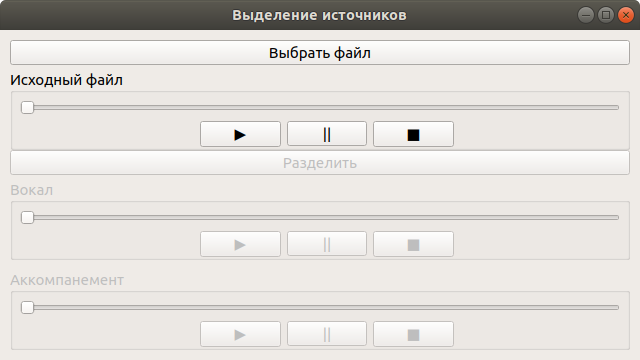
\includegraphics[width=0.8\textwidth]{inc/img/prog-main}
	\caption{Окно программы после запуска}
	\label{imp:main-window}
\end{figure}

На главном окне представлены следующие элементы:

\begin{enumerate}
	\item Кнопка <<Выбрать файл>>. Выводит окно выбора WAV-файла.
	\item Блок <<Исходный файл>>. Управляет воспроизведение исходного аудио файла. Состоит из следующих элементов:
	\begin{enumerate}
		\item Полоса прокрутки. Устанавливает момент воспроизведения, отображает процесс воспроизведения.
		\item Кнопки << $ \blacktriangleright $>>, <<||>>, <<$\blacksquare$ >> (начало воспроизведения, пауза и остановка воспроизведения соответственно). Управляют воспроизведением аудио файла.
	\end{enumerate}
	\item Кнопка <<Разделить>>. Инициализирует работу алгоритма выделения. После завершения работы метода активирует блоки <<Вокал>> и <<Аккомпанимент>> (рисунок \ref{imp:complete}).

	\item Блок <<Вокал>>. Управляет воспроизведением аудио файла голосовой составляющей. Функционал элементов соответствует блоку <<Исходный файл>>.
	\item Блок <<Аккомпанимент>>. Управляет воспроизведением аудио файла аккомпанимента. Функционал элементов соответствует блоку <<Исходный файл>>. 
\end{enumerate}


\begin{figure}
	\centering
	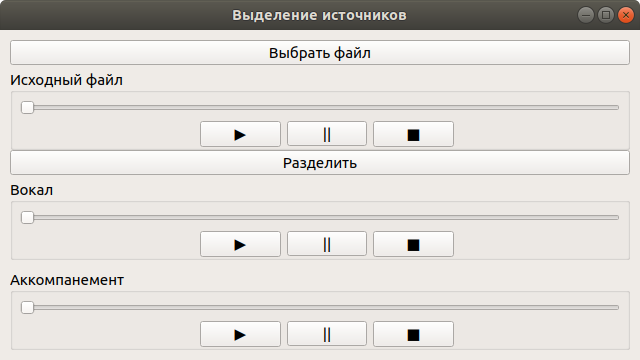
\includegraphics[width=0.8\textwidth]{inc/img/complete-window}
	\caption{Окно программы после работы метода выделения}
	\label{imp:complete}
\end{figure}

\section{Вывод}

На основе созданной архитектуры был разработан программный продукт на языке Python с использованием библиотек PyQt, TensorFlow, LibROSA и NumPy в среде PyCharm. Продукт был разработан на ЭВМ со следующими характеристиками:

\begin{itemize}
	\item Процессор: Intel Core i5.
	\item Частота процессора: 2.80GHz.
	\item Объем оперативной памяти: 8 Гб.
	\item Видеокарта: NVIDIA GeForce 840M.
	\item Операционная система: ubuntu 18.04 LTS.
\end{itemize}

Обучение нейронной сети происходило на удаленном ЭВМ со следующими характеристиками:

\begin{itemize}
	\item Количество процессоров: 2.
	\item Частота каждого из процессоров: 3.20GHz.
	\item Объем оперативной памяти: 2 Гб.
	\item Операционная система: ubuntu 16.04 LTS.
\end{itemize}

%%% Local Variables:
%%% mode: latex
%%% TeX-master: "rpz"
%%% End:

%\chapter{Экспериментальный раздел}
\label{cha:research}

В рамках дипломного проекта был проведен ряд экспериментов, направленных на исследование метода выделения голосовой составляющей из монофонического аудио сигнала. 

В качестве входных данных использовались музыкальные композиции с мужским и женским вокалом. Так же аккомпанимент мог быть записан либо с использованием музыкальных инструментов, либо при помощи цифровой звуковой рабочей станции.

\section{Описание используемой модели}

Обучение модели было произведено один раз за 150 эпох. Данный процесс занял 20 дней. Для обучения использовалась обучающая часть набора данных DSD100. График изменения ошибки в процессе обучения представлен на рисунке \ref{res:loss}.

\begin{figure}
	\centering
	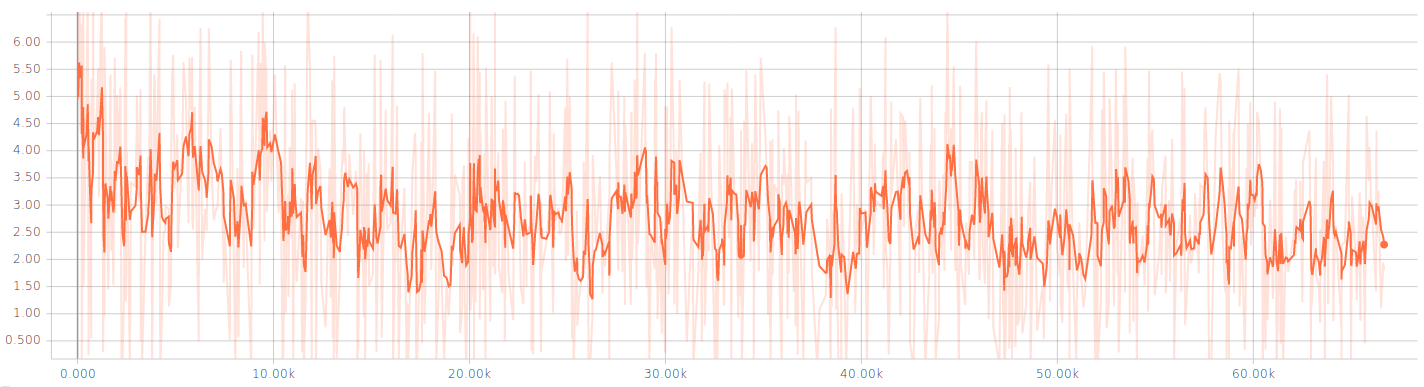
\includegraphics[width=\textwidth]{inc/img/loss-dsd}
	\caption{График изменения ошибки}
	\label{res:loss}
\end{figure}

\section{Описание тестирующей выборки}

Набор данных DSD100 состоит как из данных для обучения нейронной сети, так и из данных для ее проверки.  Данные из этого набора были приведены к двухканальному wav-файлу со следующей структурой:

\begin{itemize}
	\item Левый канал -- аккомпанимент.
	\item Правый канал -- голосовая составляющая.
\end{itemize}

\section{Методика проведения исследования}

Проведение эксперимента происходило на всей тестовой выборке набора данных DSD100. Каждый аудио файл проходил обработку разработанным методом и для полученных аудио сигналов голосовой составляющей и аккомпанемента вычислялись метрики SDR, SIR, SAR и ISR, описанные выше.

Среди полученных метрик находились максимальные и минимальные значения. На основании этих чисел определялись средние значения метрик и их разброс.

Сравнение полученных результатов с результатами методов, описанных ранее, представлено в таблице \ref{res:canonsummary}.

\begin{table}[h]
	\caption{\label{res:canonsummary}Сравнение алгоритмов выделения источников}
	\begin{center}
		\begin{tabular}{|c|c|c|c|}
			\hline
			Метод & Метрика & Вокал & Аккомпанемент \\
			\hline
			РНС & SDR & -0.6 ± 4.9 & 4.5 ± 1.2 \\
			& SIR & 1.9 ± 6.2 & 14.9 ± 5.6 \\
			& SAR & 3.6 ± 2.1 & 16.4 ± 2.9 \\
			& ISR & 7.3 ± 2.7 & 6.9 ± 1.0 \\
			\hline
			ГНС & SDR & -8.9 ± 4.4 & 4.1 ± 2.6 \\
			& SIR & 10.8 ± 3.1 & 10.7 ± 3.8 \\
			& SAR & -6.6 ± 4.6 & 12.1 ± 3.9 \\
			& ISR & 4.8 ± 2.8 & 5.0 ± 3.0 \\
			\hline
			FASST & SDR & -1.8 ± 5.8 & 8.9 ± 3.2 \\
			& SIR & -3.7 ± 7.5 & 13.7 ± 3.0 \\
			& SAR & 4.3 ± 1.4 & 13.1 ± 3.2 \\
			& ISR & 5.6 ± 2.5 & 13.5 ± 2.5 \\
			\hline
			\textbf{Глубинные РНС} & SDR & -5.6 ± 1.2 & 7.3 ± 4.2 \\
			& SIR & -3.6 ± 2.5 & 10.5 ± 1.8 \\
			& SAR & 3.8 ± 1.4 & 10.4 ± 3.2 \\
			& ISR & 5.3 ± 2.5 & 5.1 ± 2.5 \\
			\hline
		\end{tabular}
	\end{center}
\end{table} 

\section{Спектрограммы}

Были проведены сравнения спектрограмм полученных аудио сигналов с ожидаемыми. Сравнения проводились для двух музыкальных произведений: с мужским вокалом и женским вокалом.

Спектрограммы сигналов голосовой составляющей и аккомпанемента музыкального произведения с мужским вокалом представлены на рисунках \ref{res:malevoice} и  \ref{res:malemusic} соответственно.

Спектрограммы сигналов голосовой составляющей и аккомпанемента музыкального произведения с женским вокалом представлены на рисунках \ref{res:femalevoice} и  \ref{res:femalemusic} соответственно.

\begin{figure}
	\centering
	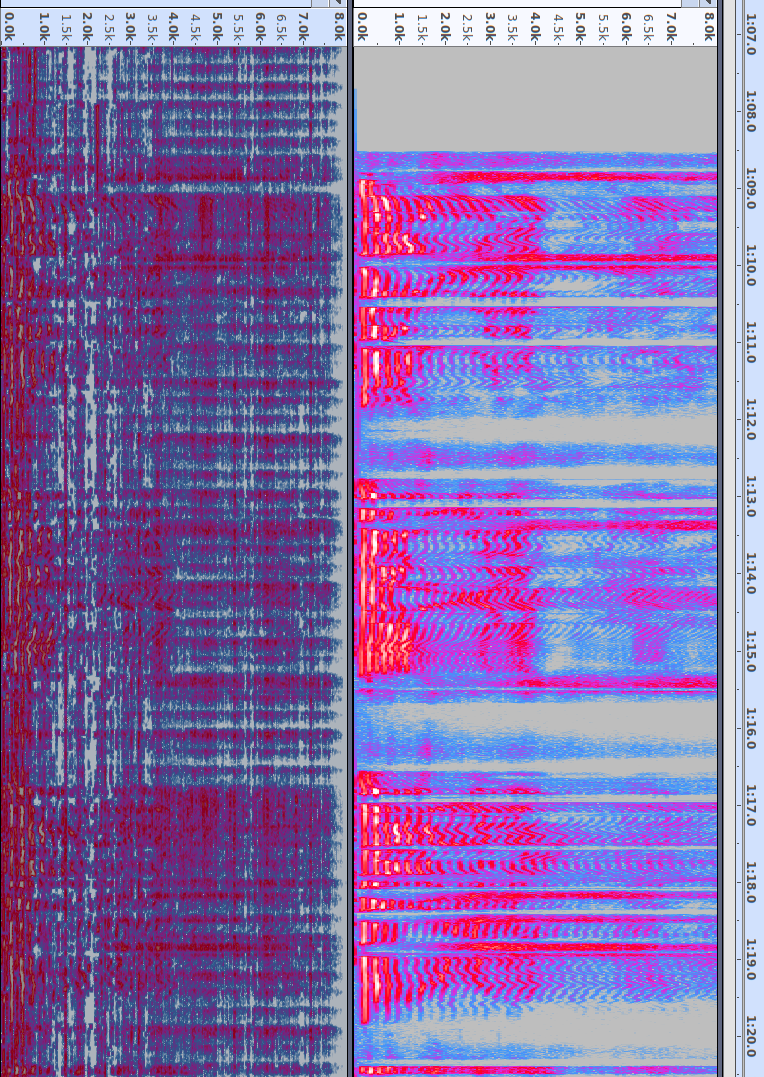
\includegraphics[width=0.9\textwidth]{inc/img/spec-voice-male}
	\caption{Сравнение спектрограмм голосовых составляющих музыкального произведения с мужским вокалом. Сверху: спектрограмма ожидаемого сигнала, снизу: спектрограмма полученного сигнала}
	\label{res:malevoice}
\end{figure}

\begin{figure}
	\centering
	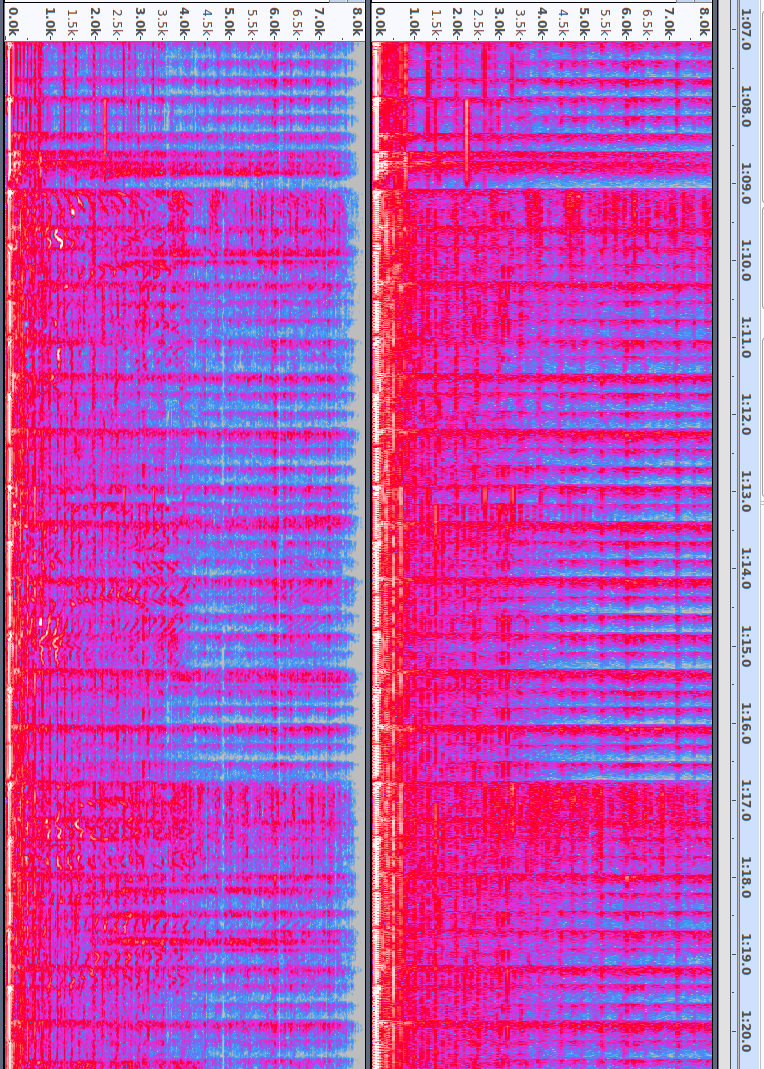
\includegraphics[width=0.9\linewidth]{inc/img/spec-music-male}
	\caption{Сравнение спектрограмм аккомпанемента музыкального произведения с мужским вокалом. Сверху: спектрограмма ожидаемого сигнала, снизу: спектрограмма полученного сигнала}
	\label{res:malemusic}
\end{figure}

\begin{figure}
	\centering
	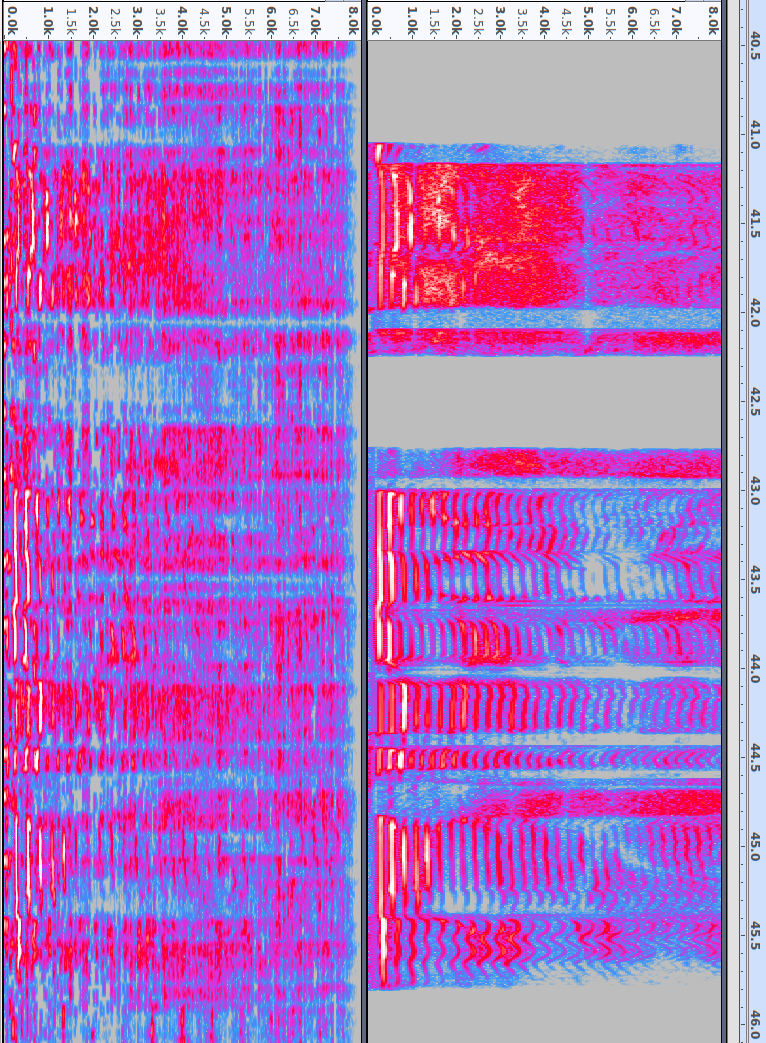
\includegraphics[width=0.9\textwidth]{inc/img/spec-voice-female}
	\caption{Сравнение спектрограмм голосовых составляющих музыкального произведения с женским вокалом. Сверху: спектрограмма ожидаемого сигнала, снизу: спектрограмма полученного сигнала}
	\label{res:femalevoice}
\end{figure}

\begin{figure}
	\centering
	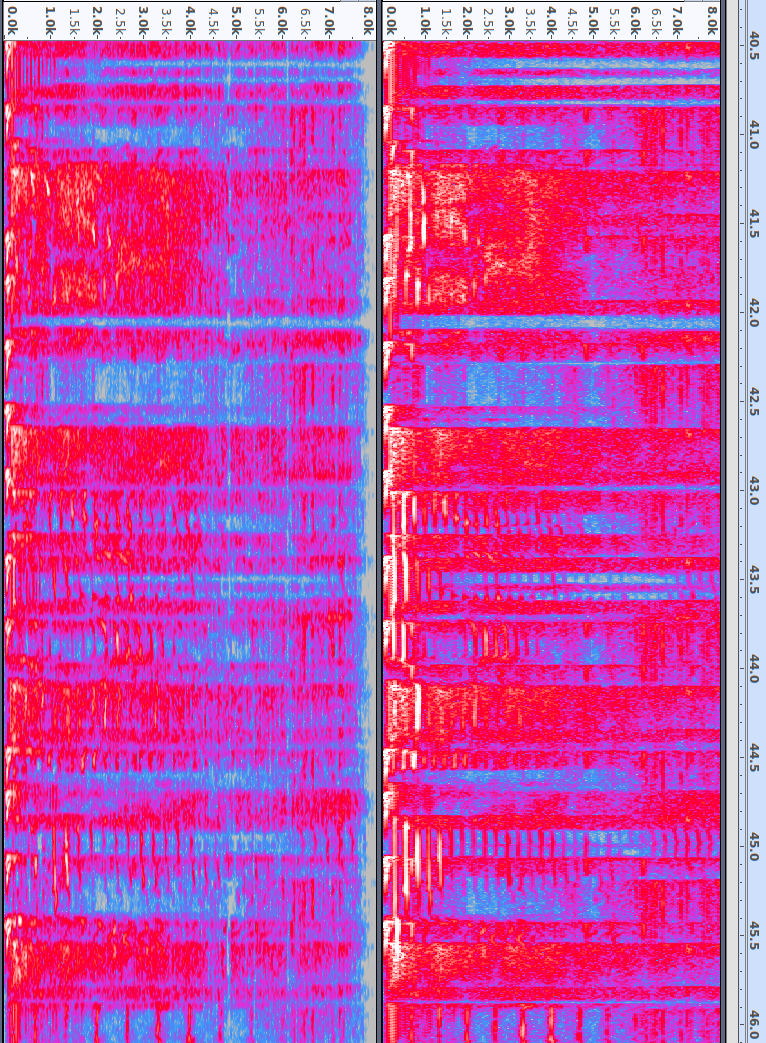
\includegraphics[width=0.9\textwidth]{inc/img/spec-music-female}
	\caption{Сравнение спектрограмм аккомпанемента музыкального произведения с женским вокалом. Сверху: спектрограмма ожидаемого сигнала, снизу: спектрограмма полученного сигнала}
	\label{res:femalemusic}
\end{figure}


%%% Local Variables:
%%% mode: latex
%%% TeX-master: "rpz"
%%% End:


\backmatter %% Здесь заканчивается нумерованная часть документа и начинаются ссылки и
            %% заключение

%\Conclusion % заключение к отчёту

В результате проделанной работы были решены следующие задачи:

\begin{itemize}
	\item был проведен анализ предметной области;
	\item были проанализированы существующие решения;
	\item на основе полученных во время анализа данных был разработан собственный метод выделения голосовой составляющей из монофонического аудио сигнала;
	\item предложенный метод был реализован в программном продукте.
\end{itemize}

В результате тестирования и эксперимента было установлено, что разработанный метод:

\begin{itemize}
	\item для вокала имеет примерно те же показатели метрик, что и метод FASST, при этом имея в среднем в два раза меньший разброс, для аккомпанемента же средние значения метрик в среднем на 60\% лучше, имея примерно те же значения разброса;
	\item для вокала значение метрик в среднем на 80\% лучше, чем у метода ГНС, при этом дисперсия в среднем в два раза меньше. Для аккомпанемента значение средних метрик приблизительно одинаков, но значение дисперсии у разработанного метода на 30\% меньше;
	\item для вокала значение метрик в среднем в 2,5 раза уступают методу СНС, при этом дисперсия в среднем в 2 раза лучше. Для аккомпанемента метрики примерно одинаковые, но разброс у разработанного метода в среднем в 2 раза больше, чем у метода СНС.
\end{itemize}

В результате тестирования и эксплуатации разработанного ПО заменен основной недостаток -- наличие примесей из соседних источников в выделяемом сигнале

Развитие разработанного метода можно осуществлять по следующим направлениям:

\begin{itemize}
	\item увеличение качества выделения переработкой архитектуры сети;
	\item определение источников, участвовавших в записи исходного сигнала.
\end{itemize}

%%% Local Variables: 
%%% mode: latex
%%% TeX-master: "rpz"
%%% End: 


% % Список литературы при помощи BibTeX
% Юзать так:
%
% pdflatex rpz
% bibtex rpz
% pdflatex rpz

\bibliographystyle{gost780u}
\bibliography{rpz}

%%% Local Variables: 
%%% mode: latex
%%% TeX-master: "rpz"
%%% End: 


%\appendix   % Тут идут приложения

%\chapter{Рисунки}
\label{cha:appendix1}



%%% Local Variables: 
%%% mode: latex
%%% TeX-master: "rpz"
%%% End: 

%\chapter{Еще картинки}
\label{cha:appendix2}

\begin{figure}
\centering
\caption{Еще одна картинка, ничем не лучше предыдущей. Но надо же как-то заполнить место.}
\end{figure}

%%% Local Variables: 
%%% mode: latex
%%% TeX-master: "rpz"
%%% End: 


\end{document}

%%% Local Variables:
%%% mode: latex
%%% TeX-master: t
%%% End:
